\chapter{Case study: Classification of SAR Textures}\label{chapter:SARclassification}

We present a newly proposed technique for texture analysis and classification based on the Bandt-Pompe symbolization for SAR data.
It consists of
(i)~linearize a \mbox{2-D} patch of the image using the Hilbert-Peano curve,
(ii)~build the Ordinal Pattern Transition Graph;
(iii)~obtain a probability distribution function derived from this graph;
(iv)~compute Information Theory descriptors (Permutation Entropy and Statistical Complexity) from this distribution and use them as features to feed a classifier.
The ordinal pattern graph we propose considers that the edges' weight is related to the absolute difference of observations, which encodes the information about the data amplitude. 
This modification considers the unfavorable signal-to-noise ratio of SAR images and leads to the characterization of several types of textures.
Experiments with data from Munich urban areas, Guatemala forest regions, and Cape Canaveral ocean samples show the effectiveness of our technique in homogeneous areas, achieving satisfactory separability levels.
The two descriptors chosen in this work are easy and quick to calculate and are used as input for a $k$-nearest neighbor classifier.
Experiments show that this technique presents results similar to state-of-the-art techniques that employ a much larger number of features and, consequently, impose a higher computational cost.

\section{Introduction}\label{SAR:Intro}

Texture is an elusive trait.
When dealing with remotely sensed images, the texture of different patches carries relevant information that is hard to quantify and transform into useful and parsimonious features.
This may be since textures, in this context, is a synesthesia phenomenon that triggers tactile responses from visual inputs.
This work presents a new way of extracting features from textures, both natural and resulting from anthropic processes, in SAR (Synthetic Aperture Radar) imagery.

SAR systems are a vital source of data because they provide high-resolution images in almost all weather and day-night conditions.
They provide basilar information, complementary to that offered by sensors that operate in other regions of the electromagnetic spectrum, for a variety of Earth Observation applications.	
Although they present rich information, such data have challenging characteristics.
Most notably, they do not follow the usual Gaussian additive model, and the signal-to-noise ratio is usually low.

\cite{Yue2020Gaussian} provide a comprehensive account of how the physical properties of the target are translated into first- and second-order statistical properties of SAR intensity data.
There is general agreement that non-deterministic textures are encoded in the second-order features, i.e., in the spatial correlation structure.
Therefore is frequent the use of covariance matrix and other measures that assume that a linear dependence, namely the Pearson correlation coefficient, suffices to characterize natural textures.
However, in SAR imagery, texture is often visible only over large areas, and the multiplicative and non-Gaussian nature of speckle antagonizes with the additive assumption that underlies classical approaches, making complex the process of characterizing such data.

Surface classification and land use are among the most critical applications of the Synthetic Aperture Radar (SAR) image~\cite{Pottier2004Unsupervised}.
In recent years, handcrafted features and representation learning (supervised and unsupervised) algorithms have been proposed~\cite{han2020unsupervised, huang2020classification, xie2020polsar}.
Algorithms of the unsupervised generative adversarial network (GAN) have revolutionized the classification of SAR images, improving performance in small sample problems, and helping the interpretability of such data~\cite{liu2019task}.
Among the supervised algorithms, support vector machine (SVM)~\cite{sukawattanavijit2017ga}, random forest (RF)~\cite{mcnairn2014early}, and neural network (NN)~\cite{lin2017deep} have been frequently used in remote sensing.
The Principle Component Analysis (PCA)~\cite{ressel2015neural}, autoencoder~\cite{wang2019classification} and the Boltzmann machine~\cite{qin2017object} can to extract non-local resources and classify non-labeled PolSAR pixels using an unsupervised approach.
However, methods such as graph-based semi-supervised deep learning algorithms~\citep{bi2018graph} can improve classification accuracy in problems with few labeled samples.

Handcrafted features in SAR textures can be studied following two complementary approaches, namely analyzing the marginal properties of the data (first-order statistics), and observing their spatial structure~\cite{Yue2020Gaussian, numbisi2018multi}.
In this work, we focus on the second approach, which shows relevant results using techniques from the image processing literature, such as co-occurrence matrices and Haralick's descriptors~\cite{yu2019detection}.
Through the gray-level co-occurrence matrices (GLCM), we can extract features that reflect statistical relationships of the pixel intensity values.
On the other hand, Haralick's descriptors can capture information on intensity and amplitude based on global statistics of SAR images.
Radford et al.~\cite{radford2018geological} used textural information derived from GLCM, along with Random Forests, for geological mapping of remote and inaccessible localities; the authors obtained a classification accuracy of $\approx\SI{90}{\percent}$, even when using limited training data ($\approx\SI{0.15}{\percent}$ of the total data). 	
Hagensieker and Waske~\cite{hagensieker2018evaluation} evaluated the synergistic contribution of multi-temporal L-, C-, and X-band data to tropical land cover mapping, comparing classification outcomes of ALOS-2~\cite{kankaku2013alos}, RADARSAT-2~\cite{morena2004introduction}, and TerraSAR-X~\cite{breit2009terrasar} datasets for a study site in the Brazilian Amazon using a wrapper approach. 
The wrapper utilizes the gray-level co-occurrence matrix texture information and a  Random Forest classifier to estimate scene importance. 	
Storie~\cite{storie2018urban} proposed an open-source workflow for detecting and delineating the urban-rural boundary using Sentinel-1A SAR data.
The author used a combination of GLCM information and a k-means classifier to produce a three-category map that distinguishes urban from rural areas. 
In higher resolution image classification activities, it is necessary to obtain more granular information from the data by extracting local characteristics such as scale and orientation.
In this scenario, techniques such as Fourier power spectrum~\cite{Florindo2012Fractal}, random fields~\cite{zhu2016antarctic}, Gabor filter~\cite{dumitru2014information} and wavelet transform~\cite{akbarizadeh2012new} are usually applied.

In our approach, we opt to analyze the \mbox{1-D} signals resulting from the linearization of the image samples, using non-parametric time series analysis techniques.
With this approach, we reduce the dimensionality of the data while preserving the spatial correlation structure.
Observations are then transformed into ordinal patterns with the Bandt-Pompe symbolization.
We use Information Theory descriptors to analyze the distributions these patterns induce, both directly and by building transition graphs among subsequent patterns.
Those descriptors are the Entropy and the Statistical Complexity, which are easy to obtain and are interpretable.
They reveal important features of the underlying process.

The following question guides us:
\begin{quote}
What is the best representation of a texture patch that allows extracting expressive Information Theory descriptors to characterize textures in the presence of speckle?
\end{quote}

Thus, we use the Weighted Amplitude Transition Graph (WATG), incorporating the absolute difference among observations as weights of the edges between nodes transitions.
Such weights take part in the computation of the probabilities and, thus, influence both Entropy and Statistical Complexity.

This work's main contribution is the proposal of a new representation of SAR textures, which allows a low-dimensional characterization useful for, among other applications, their classification.
We compare its performance with the classical histograms of Bandt-Pompe ordinal patterns and the regular transition graph.
Since the proposed approach has a low computational cost, the results obtained suggest that this technique has good potential in other applications, such as texture segmentation tools of SAR images.

\section{Linearization of image patches}\label{linearization}

We perform a data dimensionality reduction by turning the \mbox{2-D} patch into a \mbox{1-D} signal.
This could be accomplished by reading the data by lines, columns, or any transformation of \mbox{2-D} indexes into a sequence of integers.
In this work, we chose to use the Hilbert-Peano~\cite{Lee1994Texture} curve, due to its low computational cost and its ability to preserve relevant properties of pixel spatial correlation.

Nguyen et al.~\cite{nguyen1982space} firstly employed Space-filling curves, to map texture into a one-dimensional signal.
Carincotte et al.~\cite{Carincotte2006changeDetection} used the Hilbert-Peano curve in the problem of change detection in pairs of SAR images.
The authors noted that this transformation exploits the spatial locality and that its pseudo-randomness
of direction changes work well for a large family of images, especially
natural ones.

Assuming an image patch is supported by an $M \times N$ grid, we have the following definition.

\newtheorem{mydef}{Definition}
\begin{mydef}
	An image scan is a bijective function $f \colon \mathbbm{N} \times \mathbbm{N} \to \mathbbm{N}$ in the ordered pair set $ \{(i, j): 1 \leq i \leq M , 1 \leq j \leq N\}$, which denotes the points in the domain, for the closed range of integers $\{1, \dots, M  N\}$.
	A scan rule is $\{f^{-1}(1), \dots, f^{-1}(M  N)\}$.
	\label{def:CurveFilling}
\end{mydef}
This Definition imposes that each pixel is visited only once and that all pixels are visited.

Space-filling curves, such as raster-1, raster-2, and Hilbert-Peano scanning techniques, stipulate a proper function $f$.
Hilbert-Peano curves scan an array of pixels of dimension $2^k \times 2^k$, $k \in \mathbbm{N}$, never keeping the same direction for more than three consecutive points, as shown in Fig.~\ref{fig:Hilbert}.
Using the Hilbert-Peano curve, we reduce the data dimensionality while maintaining the patch's spatial dependence information.
In this work, we use Hilbert-Peano patches of size $128 \times 128$.

\begin{figure}
	\centering
	\tikz[scale=6.2] \hilbert((0mm,0mm),3);
	\hspace{0.3cm}
	\tikz[scale=2.95] \hilbert((0mm,0mm),4);
	\hspace{0.3cm}
	\tikz[scale=1.45] \hilbert((0mm,0mm),5);	
	\caption{Hilbert-Peano curves in areas of: (a)~$8 \times 8$, (b)~$16 \times 16$, and (c)~$32 \times 32$ pixels. }\label{fig:Hilbert}
\end{figure} 

Figs.~\ref{Fig:figGuatemala}, \ref{Fig:figCape1}, \ref{Fig:figCape2}, \ref{Fig:figMunich}, and~\ref{Fig:figPasture} show five image patches with different textures.
Figs.~\ref{Fig:TSGuatemala}, \ref{Fig:TSCape1}, \ref{Fig:TSCape2}, \ref{Fig:TSMunich}, and~\ref{Fig:TSPasture} present their 1-D representation as signals. 
	
\section{Methodology}\label{methodology}

Algorithm~\ref{alg:watg} outlines our methodology.
Line~\ref{Line:Peano} transforms the input texture patch $P$ in a \mbox{1-D} signal with a Hilbert-Peano sequence.
%
With this, the spatial information is encoded into a one-dimensional signal.
%
Line~\ref{Line:Probs} computes 
the probability distribution of the weighted transition graph induced by the \mbox{1-D} signal.
The WATG function is detailed in Lines~\ref{Line:WATGBegin}--\ref{Line:WATGEnd}.
%
Lines~\ref{Line:Shannon} and~\ref{Line:StatisticalComplexity} compute the two descriptors of the patch.

The \texttt{WATG} function consists of three steps: 
(i)~each sub-sequence of size (dimension) $D$ of observations at delay $\tau$ is transformed into an ordinal pattern using the Bandt-Pompe symbolization (function \texttt{BPSymbolization}, Line~\ref{Line:BP}); 
(ii)~function \texttt{transitions} (Line~\ref{Line:Transitions}) calculates the sequence of alternations of the ordinal patterns; and 
(iii)~function \texttt{weigthGraph} (Line~\ref{Line:WG}) generates the incidence matrix of the graph using the as weights the amplitude differences between the time series elements.
Finally, the probability distribution is obtained by turning the transition matrix into a vector (Line~\ref{Line:WATGEnd}).
These steps are also depicted in Fig.~\ref{fig:WATG}.

\begin{algorithm}
	\caption{$H \times C$ point from a patch using WATG}
	\label{alg:watg}                                
	\textbf{Input:} Patch of texture $P$, dimension $D$ and time delay \textbf{$\tau$}\\
	\textbf{Output:} $H \times C$ feature
	\begin{algorithmic}[1]
		\State signal.\mbox{1-D} $\gets$ \texttt{hilbertCurve}($P$) \label{Line:Peano}
		\State Probs $\gets$ \texttt{WATG}(signal.\mbox{1-D}, D, $\tau$) \label{Line:Probs}
		\State H $\gets$ \texttt{ShannonEntropy}(Probs) \label{Line:Shannon}
		\State C $\gets$ \texttt{StatisticalComplexity}(Probs) \label{Line:StatisticalComplexity}
		\State \Return $\text{H}\times\text{C}$
		
		\vspace{0.15cm}
		
		\Function{\texttt{WATG}}{signal.\mbox{1-D}, D, $\tau$}
		\State patterns $\gets$ \label{Line:WATGBegin} \texttt{BPSymbolization}(signal.\mbox{1-D}, D, $\tau$) \label{Line:BP}
		\State transitions $\gets$ \texttt{transitions}(patterns) \label{Line:Transitions}
		\State graph $\gets$ \texttt{weigthGraph}(signal.\mbox{1-D}, transitions) \label{Line:WG}
		\State Probs $\gets$ \texttt{as.vector}(graph) \label{Line:WATGEnd}
		\State \Return Probs
		\EndFunction
	\end{algorithmic}
\end{algorithm}

\begin{figure}
	\centering
	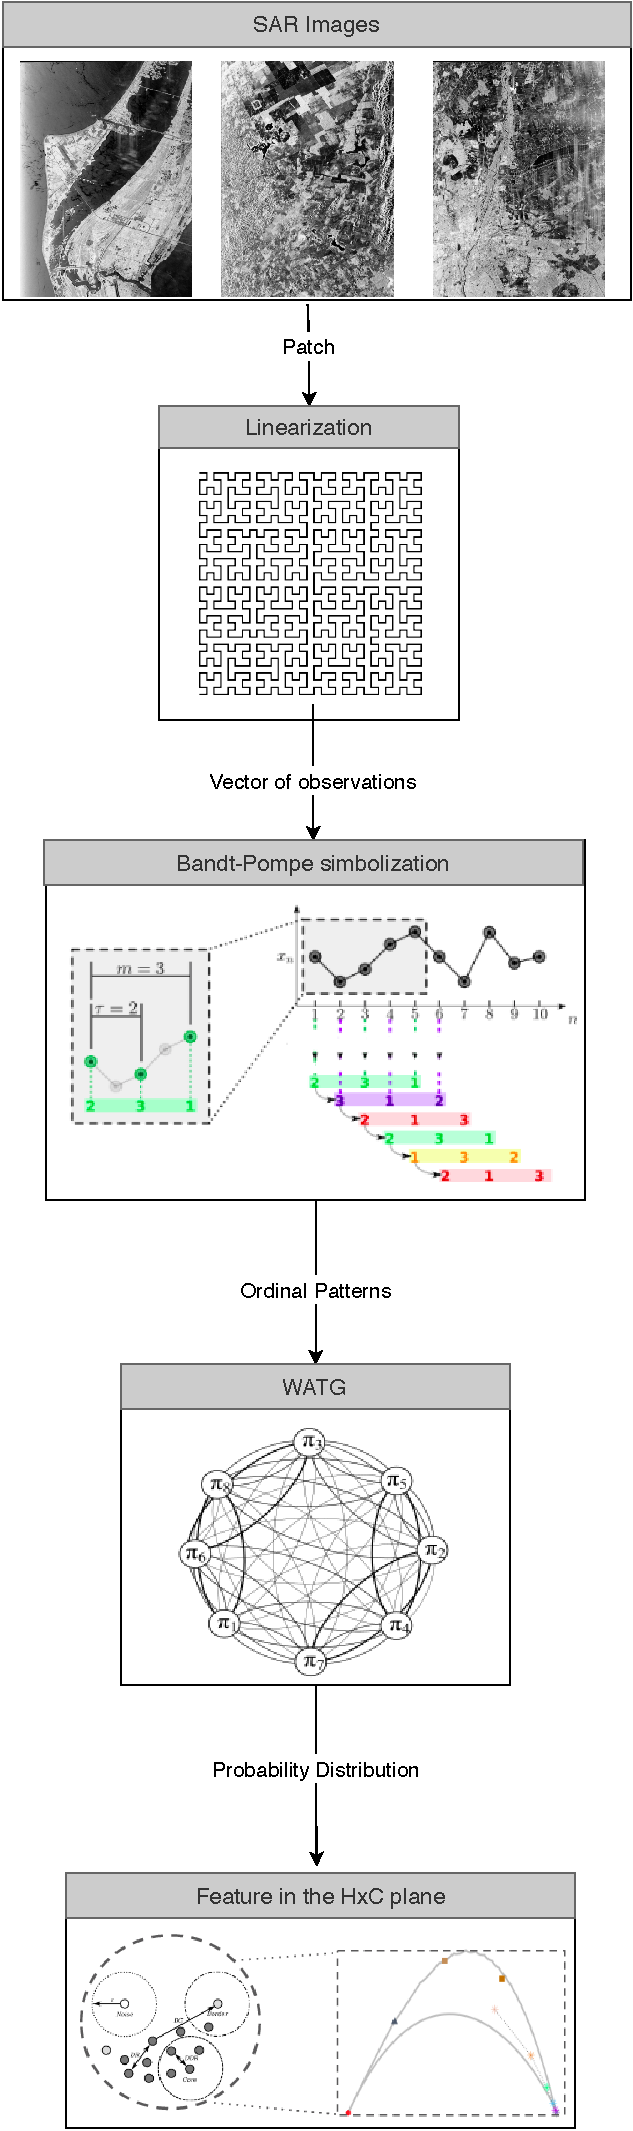
\includegraphics[width=.4\textwidth]{Figures/MethodologySAR.pdf}
	\caption{Outline of the methodology used for the classification of textures.}
	\label{fig:WATG}
\end{figure}

\section{Image Dataset}

We used the HH backscatter magnitudes of three quad-polarimetric L-band SAR images from the NASA Jet Propulsion Laboratory’s (JPL’s) uninhabited aerial vehicle synthetic aperture radar (UAVSAR) sensor with $L=36$ nominal looks:
\begin{itemize}
	\item forest and pasture region of Sierra del Lacandón National Park, Guatemala, (acquired on April 10, 2015)\footnote{\protect{\url{https://uavsar.jpl.nasa.gov/cgi-bin/product.pl?jobName=Lacand_30202_15043_006_150410_L090_CX_01\#dados}}}. 
	The image has $8917 \times 3300$ pixels with 
	\SI[inter-unit-product =$\cdot$]{10}{\meter} $\times$ \SI[inter-unit-product =$\cdot$]{2}{\meter} resolution.
	%
	\item ocean regions from Cape Canaveral Ocean (acquired on September 22, 2016).
	The image has $7038 \times 3300$ pixels with 
	\SI[inter-unit-product =$\cdot$]{10}{\meter} $\times$ \SI[inter-unit-product =$\cdot$]{2}{\meter} resolution;
	%
	\item urban area of the city of Munich, Germany (acquired on June 5, 2015)\footnote{\protect{\url{https://uavsar.jpl.nasa.gov/cgi-bin/product.pl?jobName=munich_19417_15088_002_150605_L090_CX_01\#data}}}.
	The image has $5773 \times 3300$ pixels with 
	\SI[inter-unit-product =$\cdot$]{10}{\meter} $\times$ \SI[inter-unit-product =$\cdot$]{3}{\meter} resolution.
\end{itemize}

We manually selected $200$ samples of size $128 \times 128$ to compose the dataset used in the experiments.
It is organized as follows:
$40$ samples from Guatemalan forest regions;
$40$ samples from Guatemalan pasture regions;
$80$ samples from the oceanic regions of Cape Canaveral, divided into two types with different contrast; and
$40$ samples of urban regions of the city of Munich.
Fig.~\ref{fig:samples&Series} shows examples of each. In our analysis, both types of ocean images are grouped.

We randomly split the samples in training (\SI{85}{\percent}) and test (\SI{15}{\percent}) sets.
We used the first set to train a $k$-nearest neighbor classifier algorithm with tenfold
cross-validation.

\begin{figure*}
	\centering
	\subfigure[Forest\label{Fig:figGuatemala}]{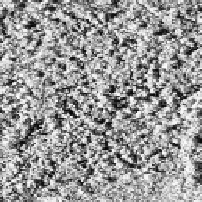
\includegraphics[width = 29mm]{Figures/guatemalaflorest.pdf}}
	\subfigure[Sea -- lower contrast\label{Fig:figCape1}]{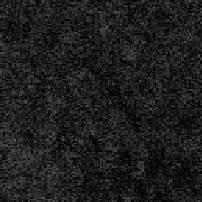
\includegraphics[width = 29mm]{Figures/Cape1.pdf}}
	\subfigure[Sea -- higher contrast\label{Fig:figCape2}]{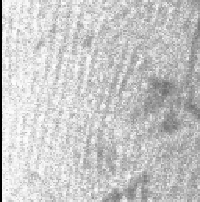
\includegraphics[width = 29mm]{Figures/Cape2.pdf}}
	\subfigure[Urban\label{Fig:figMunich}]{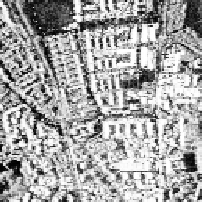
\includegraphics[width = 30mm]{Figures/munichUrban.pdf}}
	\subfigure[Pasture\label{Fig:figPasture}]{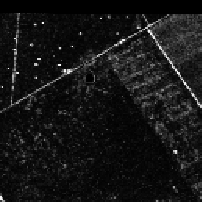
\includegraphics[width = 30mm]{Figures/pasture.pdf}}
	
	\subfigure[Signal -- forest\label{Fig:TSGuatemala}]{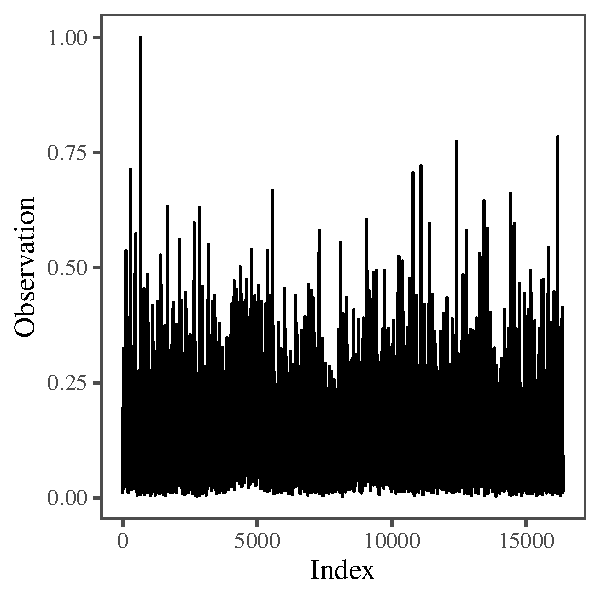
\includegraphics[width = 30mm]{Figures/tsguatemala.pdf}}
	\subfigure[Signal -- sea\label{Fig:TSCape1}]{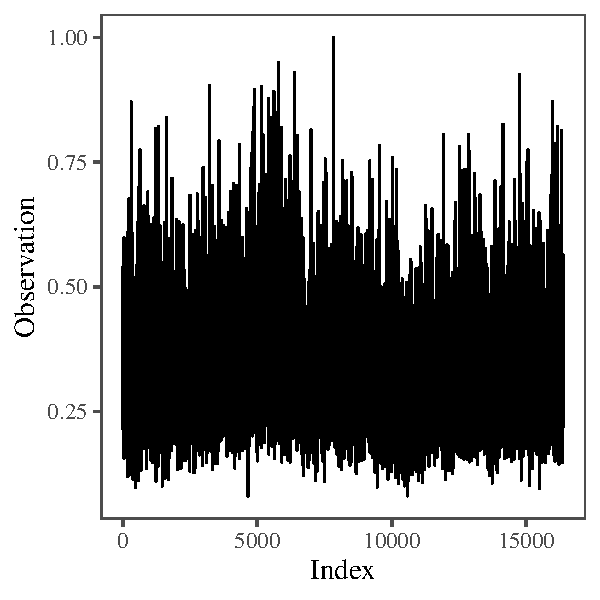
\includegraphics[width = 30mm]{Figures/tscape1.pdf}}
	\subfigure[Signal -- sea\label{Fig:TSCape2}]{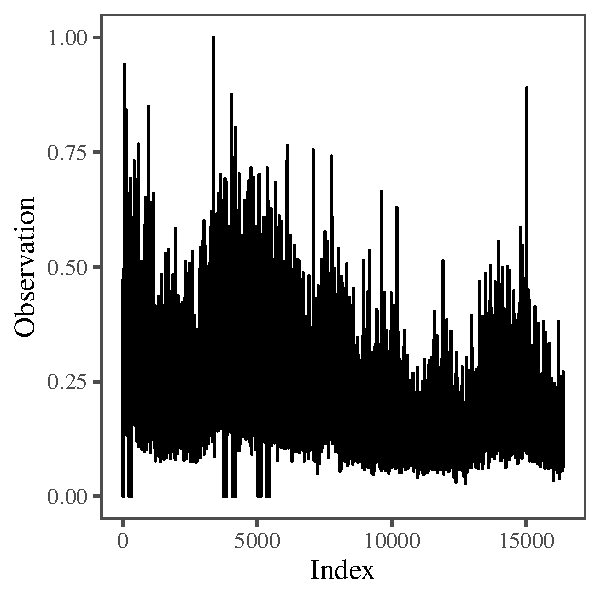
\includegraphics[width = 30mm]{Figures/tscape2.pdf}}
	\subfigure[Signal -- sea\label{Fig:TSMunich}]{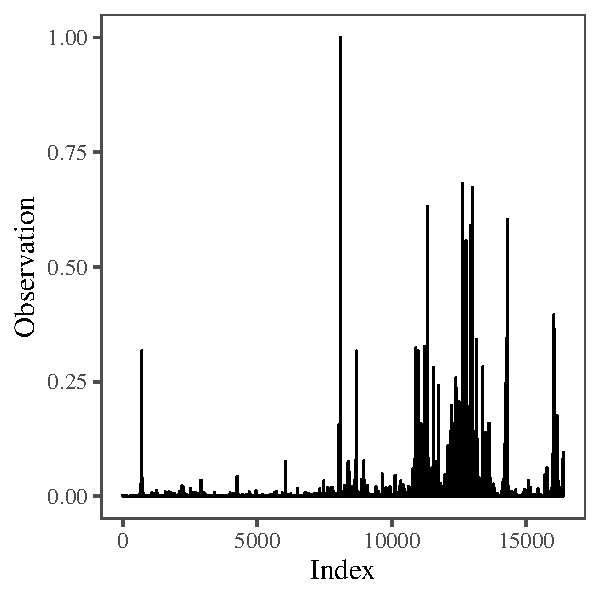
\includegraphics[width = 30mm]{Figures/tsmunich.pdf}}
	\subfigure[Signal -- pasture\label{Fig:TSPasture}]{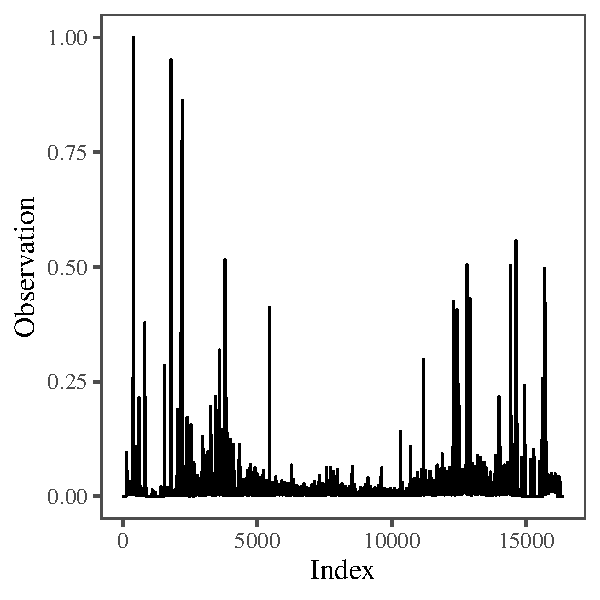
\includegraphics[width = 30mm]{Figures/tspasture.pdf}}
	\caption{Types of regions (Guatemala forest, Canaveral ocean types 1 and 2, Munich urban area, and pasture area) and their signal representation.}
	\label{fig:samples&Series}
\end{figure*}

\section{Experimental Results and Analysis}\label{Results}

In this section, we describe  the classification process, and 
the results of applying WATG.
To assess the performance of the technique here proposed, we analyze the impact of its parameters and compare its results in the classification with other methods.

\subsection{Properties}\label{Sec:WATGProperties}

We conducted two experiments to analyze the response of WATG to different noise levels and image rotations.
Our truth is the deterministic image generated by the function:
\begin{equation*}
z(x,y) = \sin (4x + 0.5y), 
\end{equation*}
where  $x, y \in [-2\pi, 2\pi]$.
Fig.~\ref{Fig:TestZ} shows this function as a $128\times128$-pixel patch.

The speckle noise was modeled as outcomes of independent, identically distributed unitary-mean Gamma random variables with shape parameter $L$ (the number of looks, which controls the signal-to-noise ratio)
$W(L) \sim \Gamma(L, L)$,
with $L \in \{1, 100, 150, 200, 250, 300, 350, 400, 450, 500\}$.
The observed images $I(L)$ are the pixelwise product of $z$ and $w(L)$.
Fig.~\ref{Fig:TestZW} shows the product $I(100)$.

\begin{figure}
	\centering
	\subfigure[$z$]{\label{Fig:TestZ}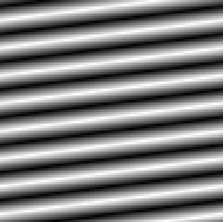
\includegraphics[width = 45mm]{Figures/z.png}}
	\subfigure[$I(100)$]{\label{Fig:TestZW}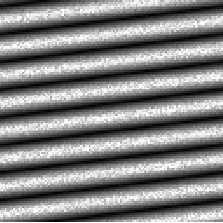
\includegraphics[width = 45mm]{Figures/z100.png}}
	\subfigure[$I^{\text{T}}(500)$]{\label{Fig:TestRot}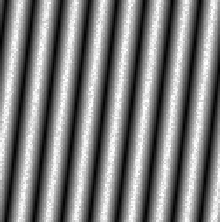
\includegraphics[width = 45mm]{Figures/z500t.png}}
	\caption{Ground truth, speckled, and speckled transposed versions.}
	\label{Fig:TestZWL}
\end{figure}

Fig.~\ref{Fig:TestSpeckleHC} shows how the point in the $H\times C$ plane varies according to the level of noise introduced.
The ground truth (identified as ``\textsf{0}'') has relatively low entropy and is close to the maximum complexity (the continuous line is the upper bound).
This behavior is typical of deterministic sequences.
Observe that when we inject single-look speckle ($L=1$), the entropy increases along with the complexity.
Thus, the technique is able to identify the deterministic component even when it is embedded in the strongest possible speckle noise.
The point ``\textsf{1}'' shifts towards ``\textsf{0}'' when the signal-to-noise progressively increases.

\begin{figure}
	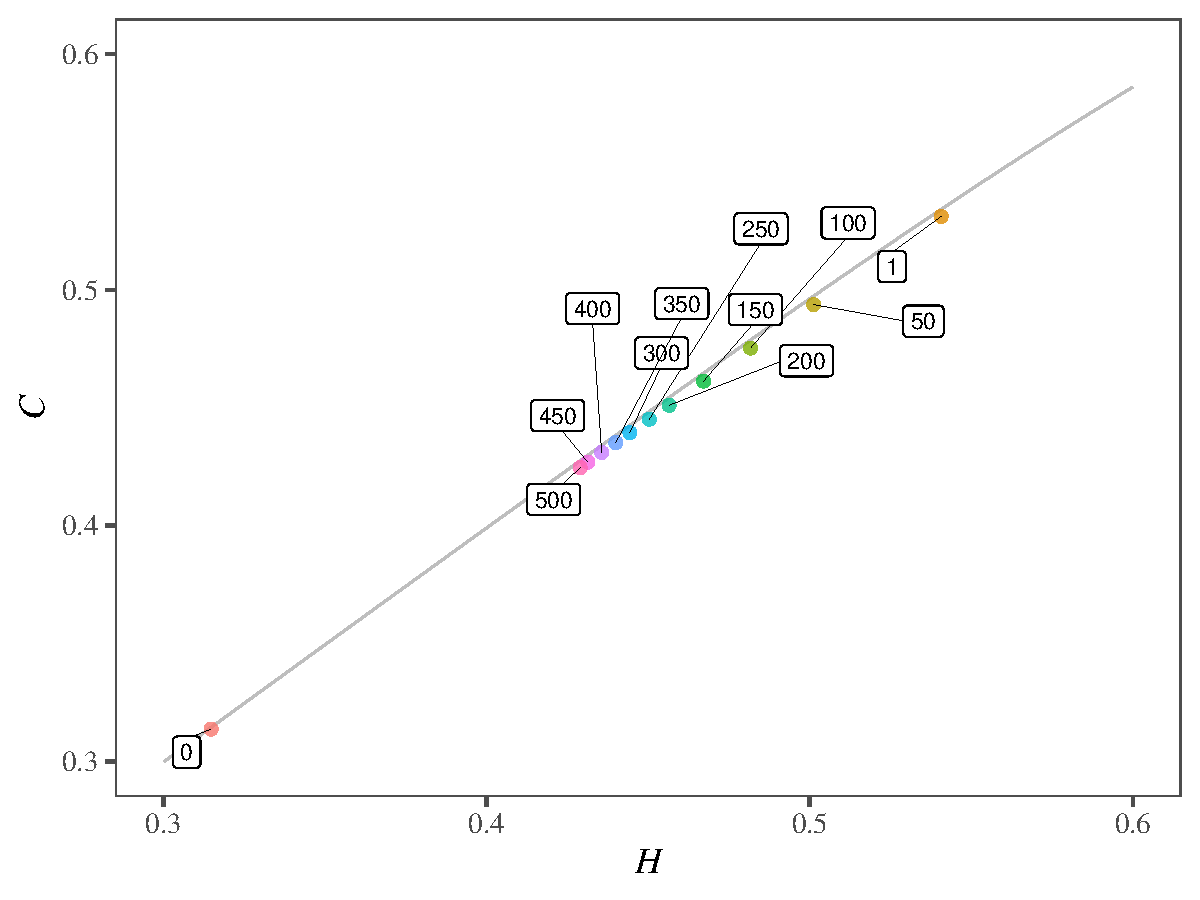
\includegraphics[width=\textwidth]{Figures/Waves1.pdf}
	\caption{Modifications to the $H \times C$ Plane features by adding different multiplicative noises.}
	\label{Fig:TestSpeckleHC}
\end{figure}

We also verified that the points in the $H\times C$ plane are almost insensitive to rotations.
Fig.~\ref{Fig:TestRot} shows the transpose of $I(500)$.
In all cases, the coordinates $(h,c)$ of the transposed noisy images were equal, up to the fourth decimal place, to those of the original version.

These experiments provide evidence that the WATG mapping is little sensitive to rotations (thanks to the use of Hilbert-Peano curves), and that it can identify the presence of underlying structural information in the presence of varying levels of speckle.


\subsection{Analysis of ordinal patterns methods}

Fig.~\ref{fig:samples&Series} shows examples of the ocean, forest, urban, and pasture both as image patches and as 1-D sequences after the linearization process.

The variation in the magnitude of the targets' backscatter and, consequently, in the intensity of the image pixels, depends on the intrinsic properties of the region under analysis.
Urban targets usually exhibit the strongest variation, followed by forest, pasture, forests, and finally, water bodies.
By adding such information related to the amplitude, the proposed method is able to increase, compared to traditional methods, the granularity of information captured by ordinal patterns.

As already described in Section~\ref{chapter:WATG}, our proposal weights the edges in terms of the difference of amplitudes.
As expected, the greatest impact is observed on the transition graphs obtained from urban areas.
The urban area \mbox{1-D} signal shown in Fig.~\ref{fig:samples&Series} has the largest dynamic range.
Fig.~\ref{fig:graphs} shows how this information alters the weights of the transition graph.
Notice, in particular, that 
$(v_{\widetilde \pi^3_{123}}, v_{\widetilde \pi^3_{123}})$ almost doubled, while 
$(v_{\widetilde \pi^3_{312}}, v_{\widetilde \pi^3_{231}})$ and $(v_{\widetilde \pi^3_{213}}, v_{\widetilde \pi^3_{132}})$ became negligible.

\begin{figure*}
	\centering
	\subfigure[Transition Graph\label{Fig:UrbanTG}]{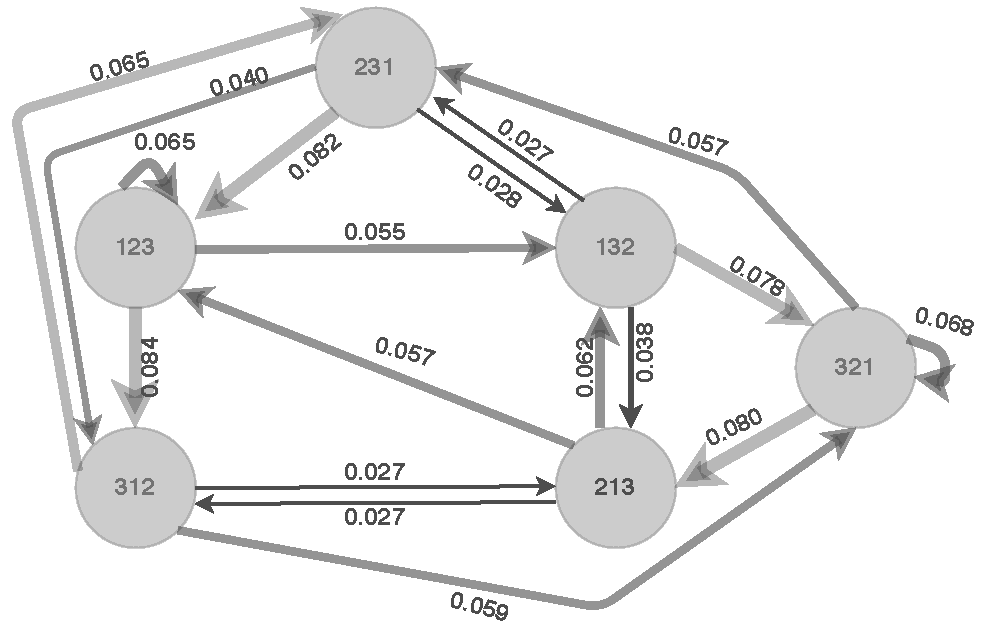
\includegraphics[width = 75mm]{Figures/UrbanTG.pdf}}
	\subfigure[WATG\label{Fig:UrbanWATG}]{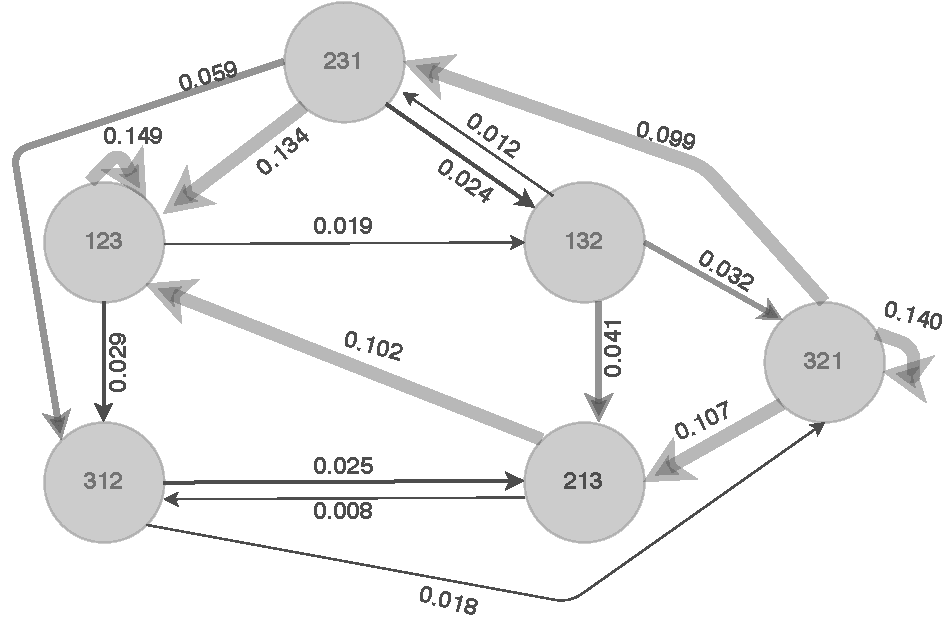
\includegraphics[width = 75mm]{Figures/UrbanWATG.pdf}}
	\caption{Difference of edges weights between the transition graph and the weighted graph of ordinal patterns transitions; urban area, with dimension 3 and delay 1.}
	\label{fig:graphs}
\end{figure*}

Fig.~\ref{fig:2DVisualization} shows the impact of using the data amplitude information on the weights of the transition graphs.
Bandt-Pompe symbolization was the first method based on ordinal patterns proposed in the literature.
As shown in Fig.~\ref{Fig:bp}, it provides limited separation of textures.
The transition graphs (Fig.~\ref{Fig:tg})improve the spread of the features, but with some amount of confusion.
Our proposal, shown in Fig.~\ref{Fig:watgD3T1}, produces well-separated features.
In this way, we were able to obtain, for this experiment, a perfect characterization and, consequently, the high descriptive power of the regions.

\begin{comment}
\begin{figure}
	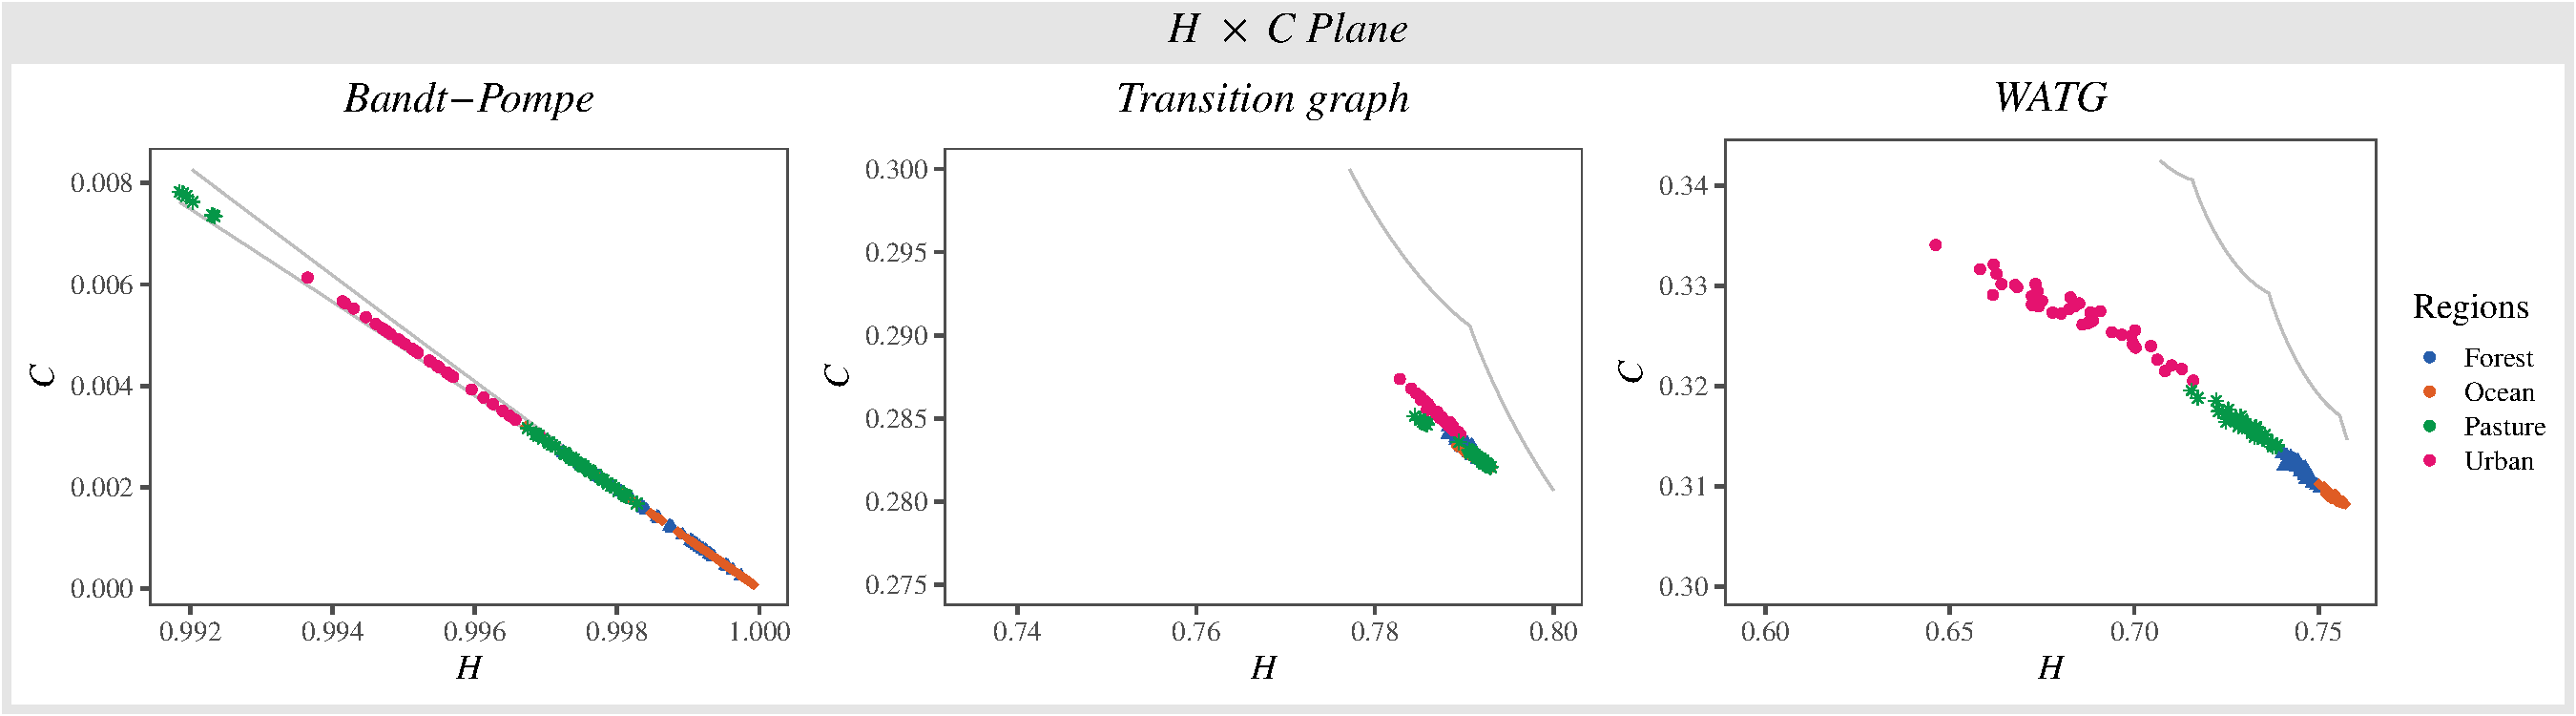
\includegraphics[width=\columnwidth]{Figures/HCAnalysis.pdf}
	\caption{Location of Guatemala (forest), Cape Canaveral (ocean), and Munich (urban) in the $H \times C$ plane for dimension 3 and delay 1. 
	The continuous curves correspond to the maximum and minimum values of $C$ as a function of $H$.}
	\label{fig:plotsHC}
\end{figure}
\end{comment}

\subsection{Experiments on sliding window selection}

In this section, we analyze the parameters of the proposed method and its impact on textures classification.
McCullough et al.~\cite{McCullough2015lagged} report that inadequate values may hinder important characteristics of the phenomenon under analysis.
The two parameters of the transition graph are the dimension $D$, and the delay $\tau$.
In the experiments below, we present the results in the classification using different values of these parameters.

The classification method's performance based on ordinal patterns is sensitive to window size, the embedding dimension, and the delay.
In techniques based in Bandt-Pompe symbolization, for a fixed signal, as the size of the embedding dimension decreases, more ordinal patterns are produced.
Therefore, we acquire a higher granularity of information about the dynamics of the system and, consequently, we capture more spatial dependencies between the elements.

Fig.~\ref{fig:ROC} shows the ROC plane for different values of $D \in \{3, 4, 5, 6 \} $ and $\tau \in \{1, 2, 3, 4, 5 \}$ to select the best configuration.
The configurations that extracted most information from the \mbox{1-D} signal and, thus, that presented the best results in the experiments, are $(D = 3, \tau = 1)$ and $(D = 4, \tau = 1)$.
The technique, thus, shows its best performance choosing the parameters with the lowest computational cost.

\begin{figure}
	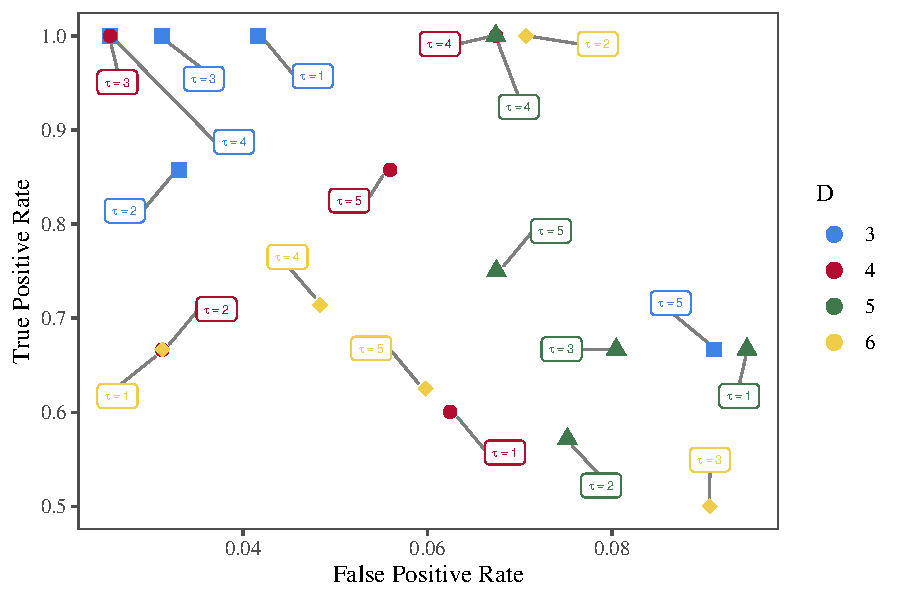
\includegraphics[width=\columnwidth]{Figures/ROC.pdf}
	\caption{Evaluation of the sliding window parameters using ROC curve}
	\label{fig:ROC}
\end{figure} 

Figure~\ref{fig:Regions} shows the points in the $H\times C$ produced by the same samples with all the parameters mentioned above.
The spatial distribution of the points changes with the parameters and specific configurations promote better separation.
This figure shows that the discrimination ability decreases with increasing $\tau$.
Larger values of delay dilute the spatial dependence, as neighboring points in the sample tend to be more distant in the image.
For this reason, we use $\tau=1$. Figure~\ref{fig:Regions} suggests that only one feature ($H$ or $C$) is sufficient to discriminate the classes studied. Although this is true for the experiments herein conducted, we opt to preserve the most common ordinal pattern analysis, which uses both features. As we studied only homogeneous patches, we still do not know how this approach performs with heterogeneous patches. %In this last case, it is necessary to detect borders to segment the images into homogeneous patches. 
For this last situation, we may need both features.

\begin{sidewaysfigure*}
	\centering
	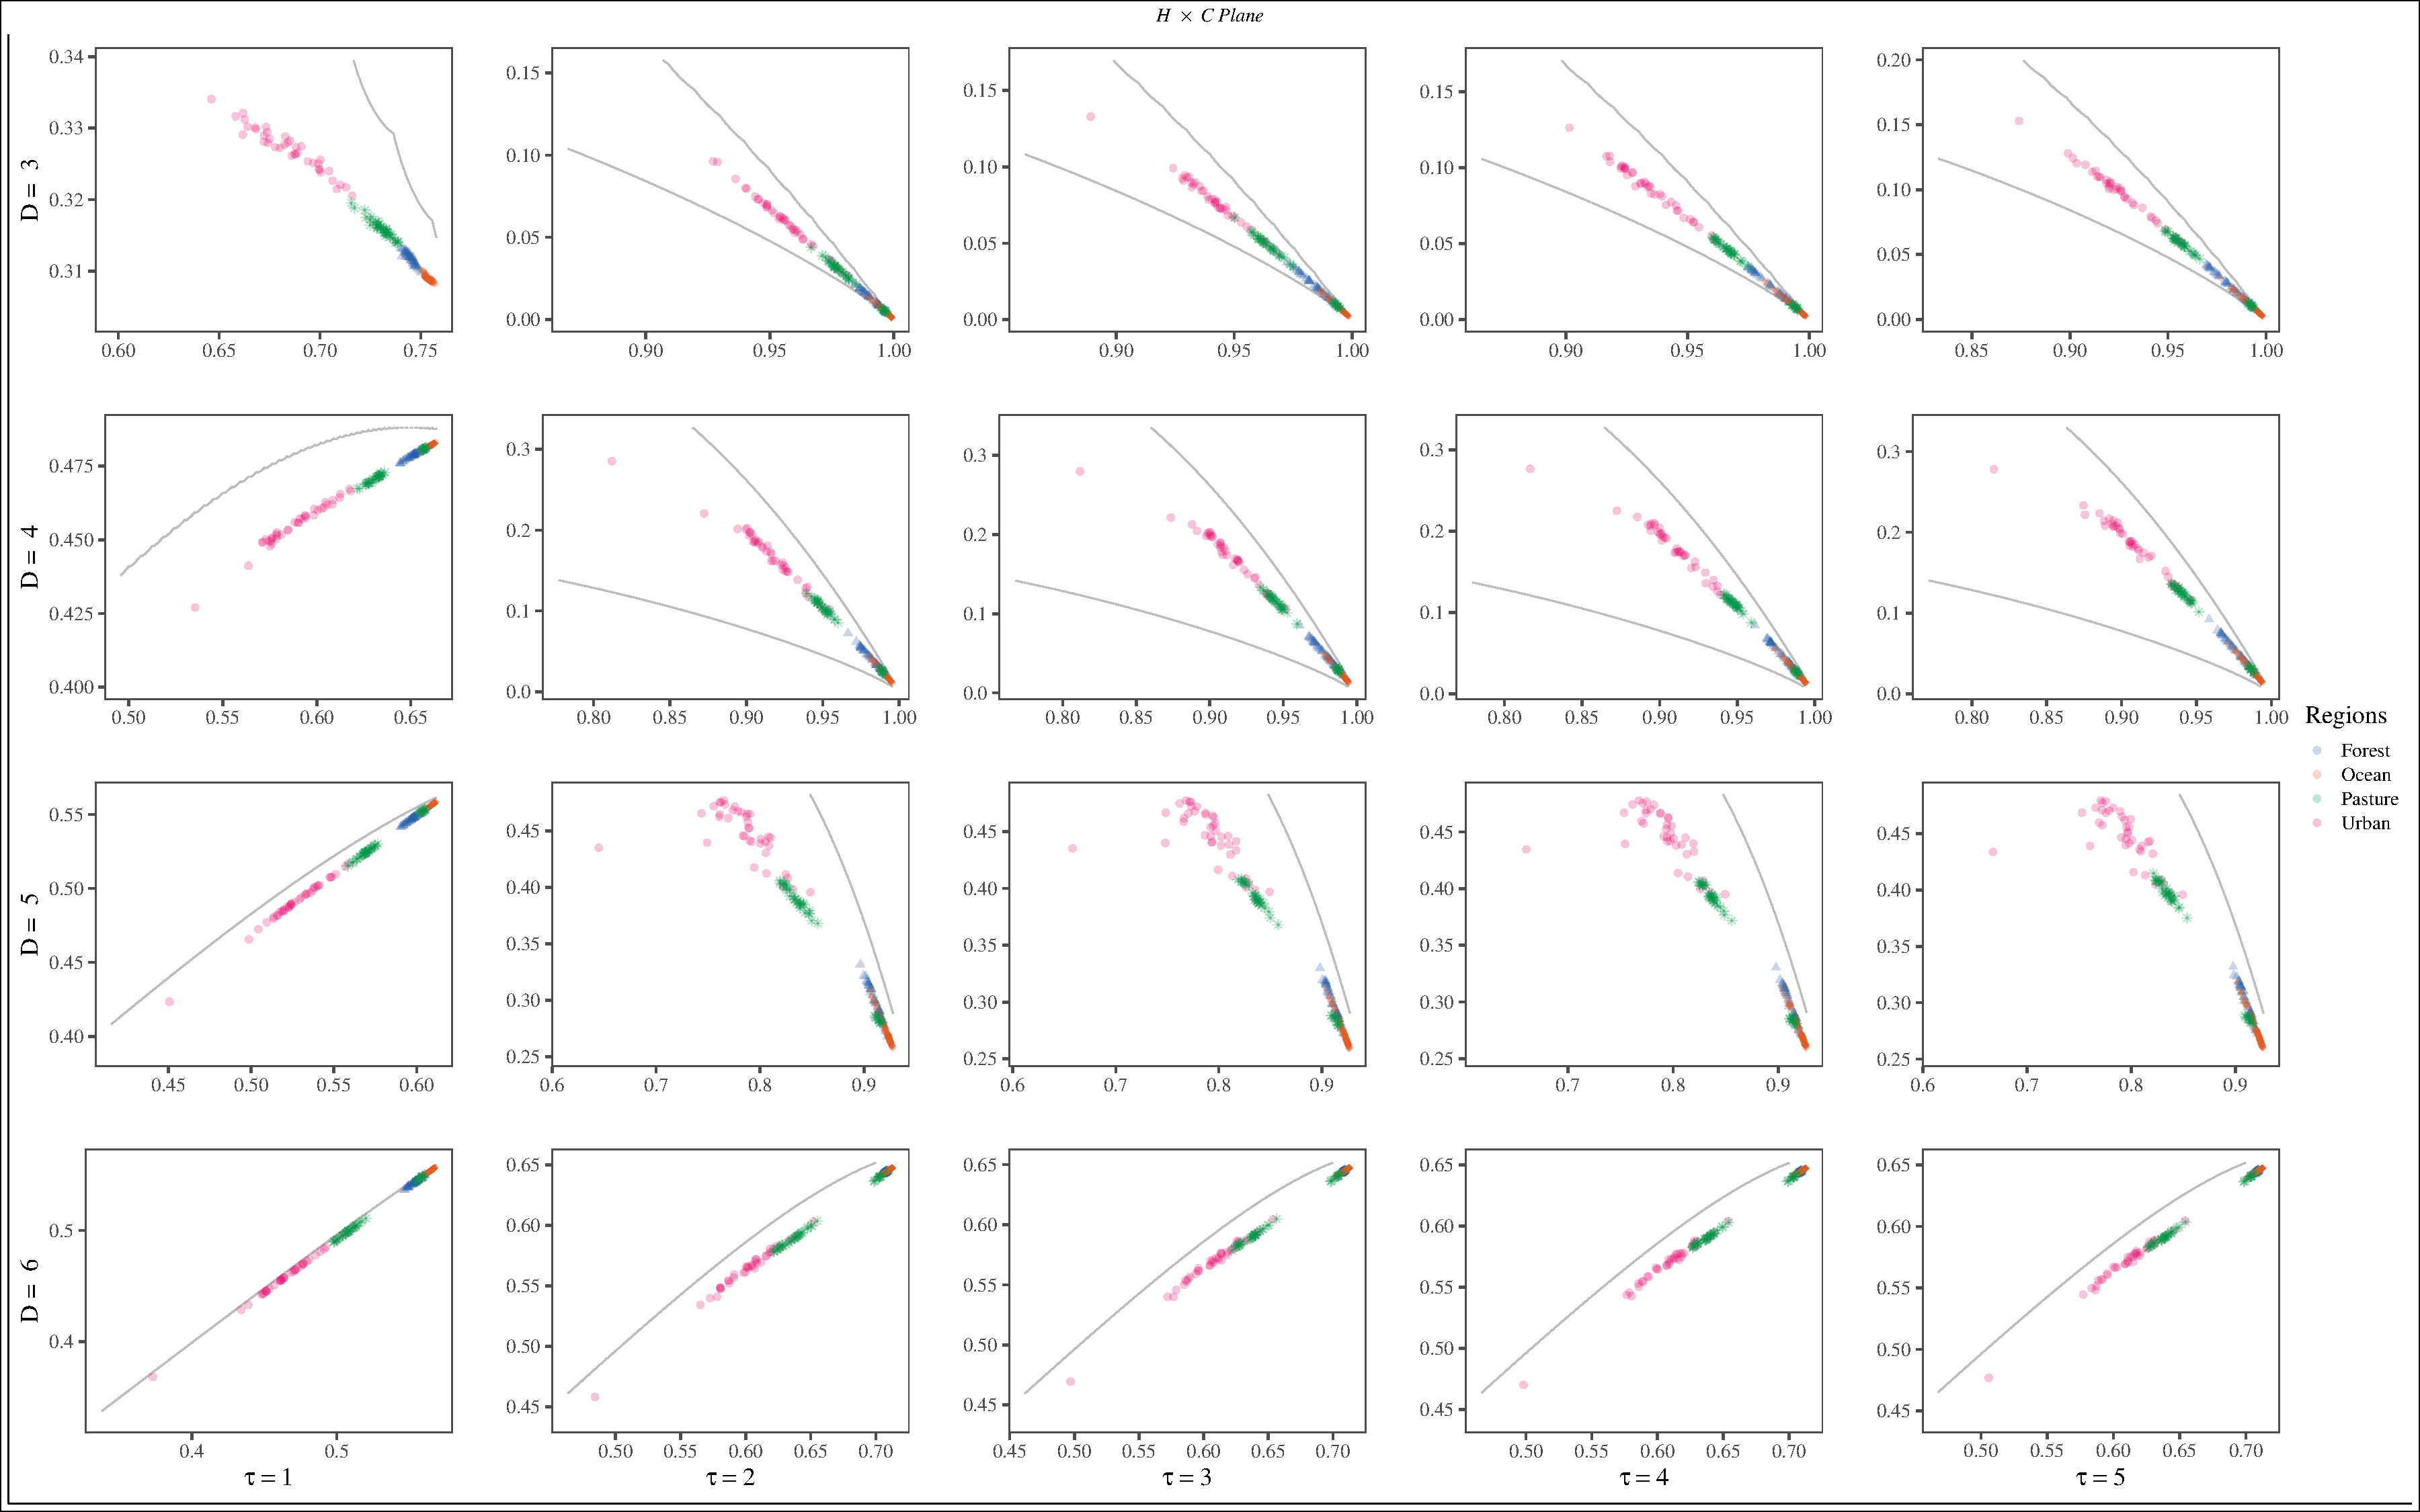
\includegraphics[width=1\textwidth]{Figures/WATGHC.pdf}
	\caption{Characterization resulting in $H \times C$ Plane from the application of the Hilbert-Peano curve in WATG on textures of different regions: Guatemala (forest), Cape Canaveral (ocean) and Munich (urban). 
	The continuous curves correspond to the maximum and minimum values of $C$ as a function of $H$.}
	\label{fig:Regions}
\end{sidewaysfigure*}

Considering $\tau=1$ (first column of Fig.~\ref{fig:Regions}), 
we also notice that $D=3$ produces the best separation among classes.
Increasing $D$ also increases the Statistical Complexity; this is noticeable for the Forest class.
The other effect of considering larger values of $ D $ is an increased Entropy of Ocean and an undesirable overlap with Urban samples.

\subsection{Quantitative Evaluation}

We present a comparison between our proposal and other methods for texture characterization and classification.
We use the following ten methods: 
Gabor filters~\cite{weldon1996efficient},  
Histogram of oriented gradients (HOG)~\cite{dalal2005histograms},
Gray-level co-occurrence matrices (GLCM)~\cite{kourgli2012texture}, 
Speeded-Up Robust Features (SURF)~\cite{bay2006surf},
Short Time Fourier Transform (STFT)~\cite{portnoff1980time} with SURF,
Bandt-Pompe probability distribution~\cite{Bandt2002Permutation}, 
Ordinal patterns transition graphs~\cite{Borges2019Transition},
Weighted Permutation Entropy (WPE)~\cite{Fadlallah2013Weightedpermutation},
Fine-Grained Permutation Entropy (FGPE)~\cite{xiao2009fine} with $\alpha = 0.5$, and
Amplitude-Aware Permutation Entropy (AAPE)~\cite{azami2016amplitude} with $A = 0.5$.
As in~\cite{guan2019covariance}, 
we computed four statistics from co-occurrence matrices: contrast, correlation, energy, and homogeneity.
Likewise, we implemented the Gabor filters in five scales and eight orientations; using the energy, we obtained an $80$-dimensional feature vector for each patch.
For the HOG technique, we used image pixels divided into equal cells of $3 \times 3$ pixels, and for each cell, we computed 6-bin histograms ranging from \SIrange{0}{180}{\degree} or \SIrange{0}{360}{\degree}.

The results of visualizing the features of these descriptors can be seen in Fig.~\ref{fig:2DVisualization}.
As we can see, the algorithms that combine ordinal characteristics with amplitude information (WPE, AAPE, and FGPE) reduce the intra-class distance, but not are good discriminators.
Although the algorithms that have the largest descriptors (Gabor and HOG) do not present a good visualization when applying the dimensionality reduction technique, they presented excellent results in the quantitative evaluation.


\begin{figure*}
	\centering
	\subfigure[Gabor Filter\label{Fig:Gabor}]{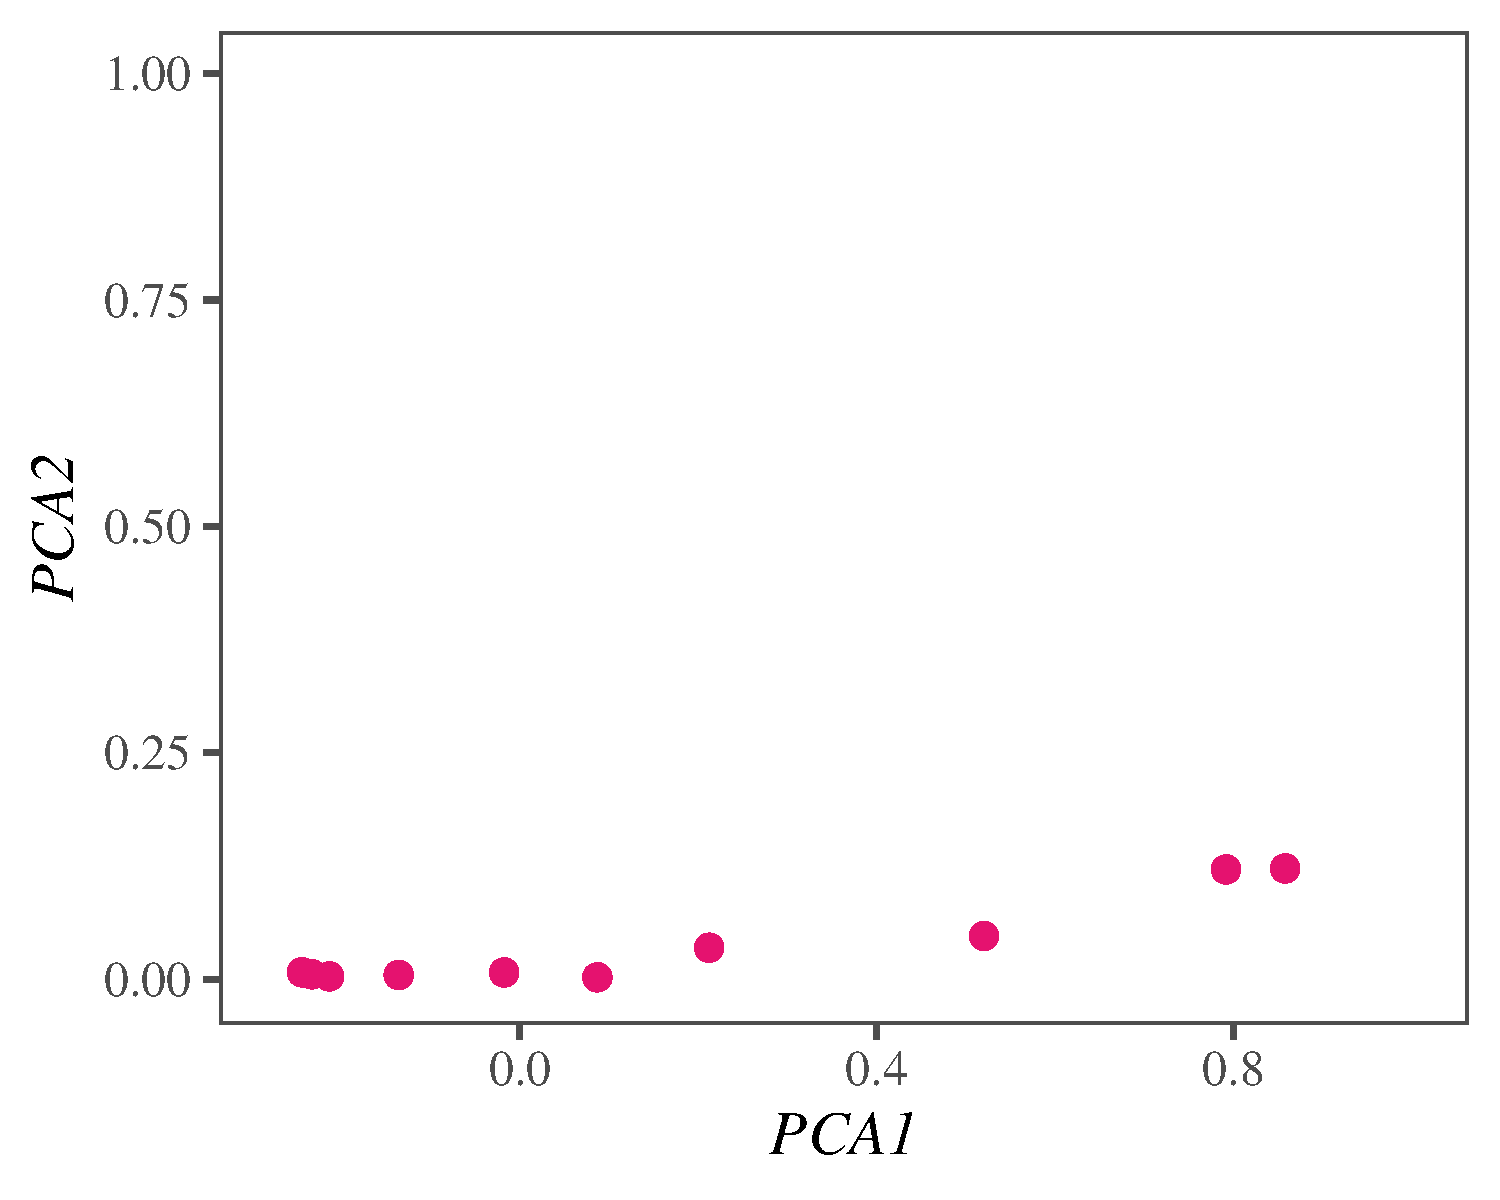
\includegraphics[width = .3\columnwidth]{Figures/Gabor.pdf}}
	\subfigure[HOG\label{Fig:hog}]{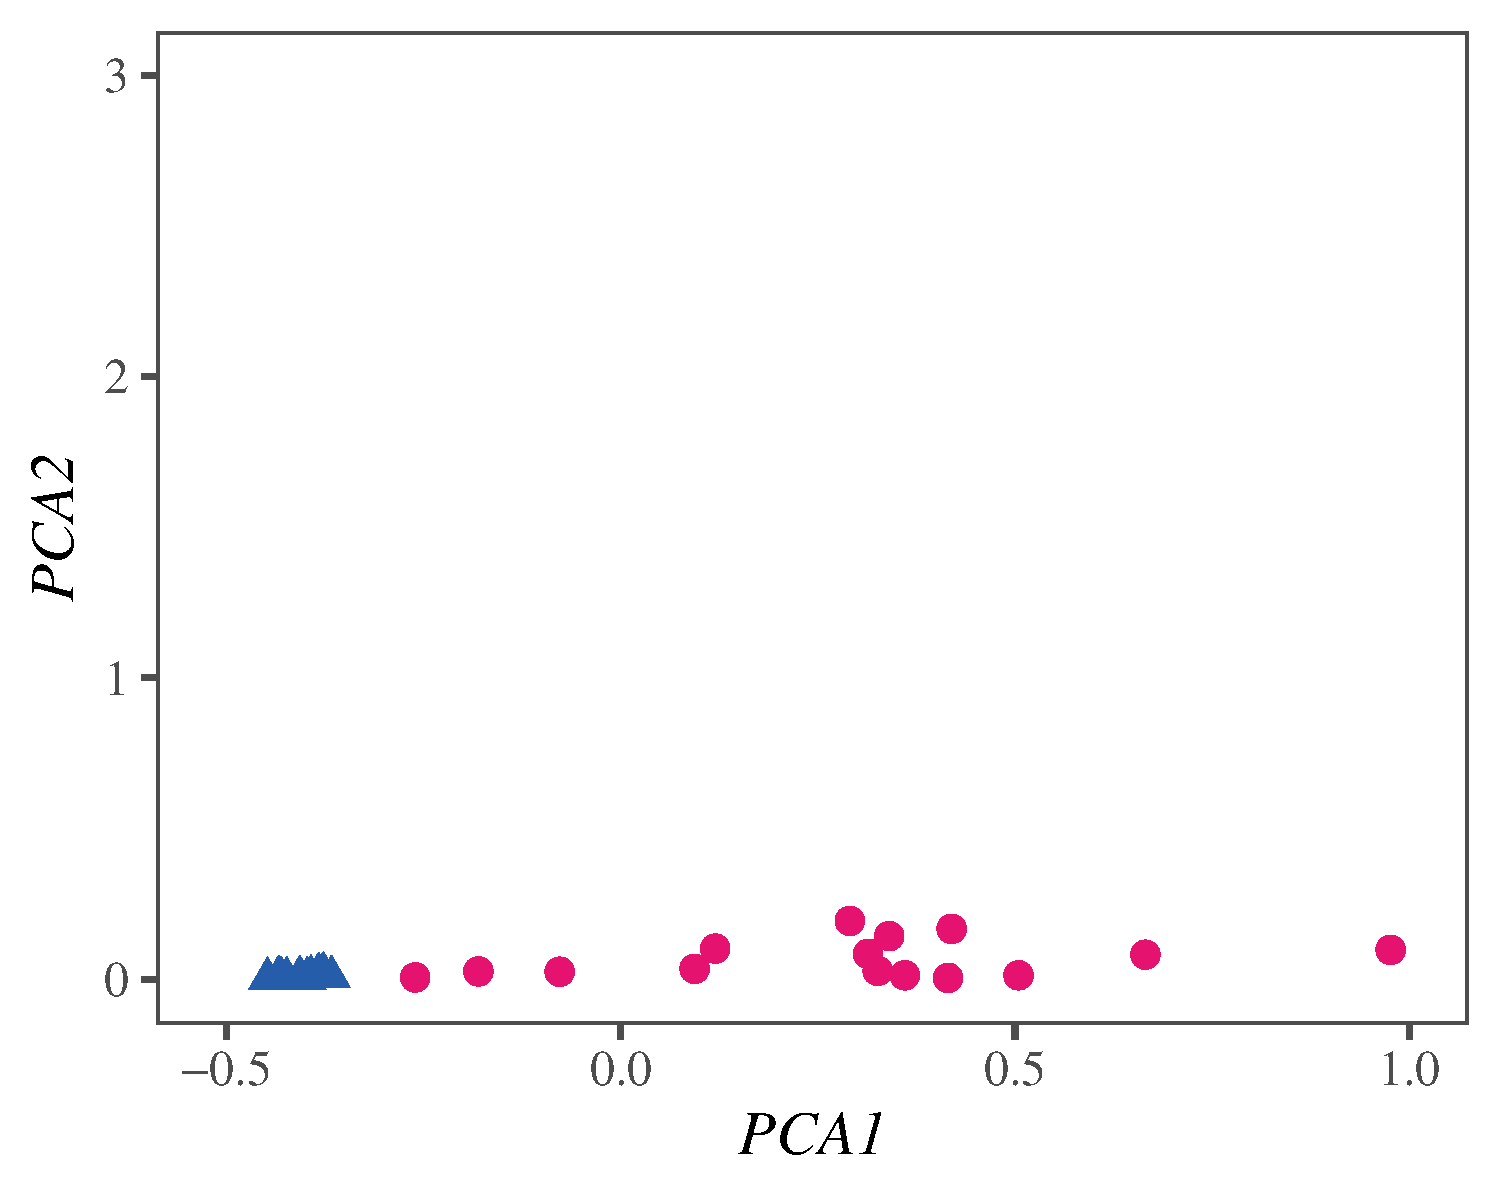
\includegraphics[width = .3\columnwidth]{Figures/HOG.pdf}}
	\subfigure[GLCM\label{Fig:glcm}]{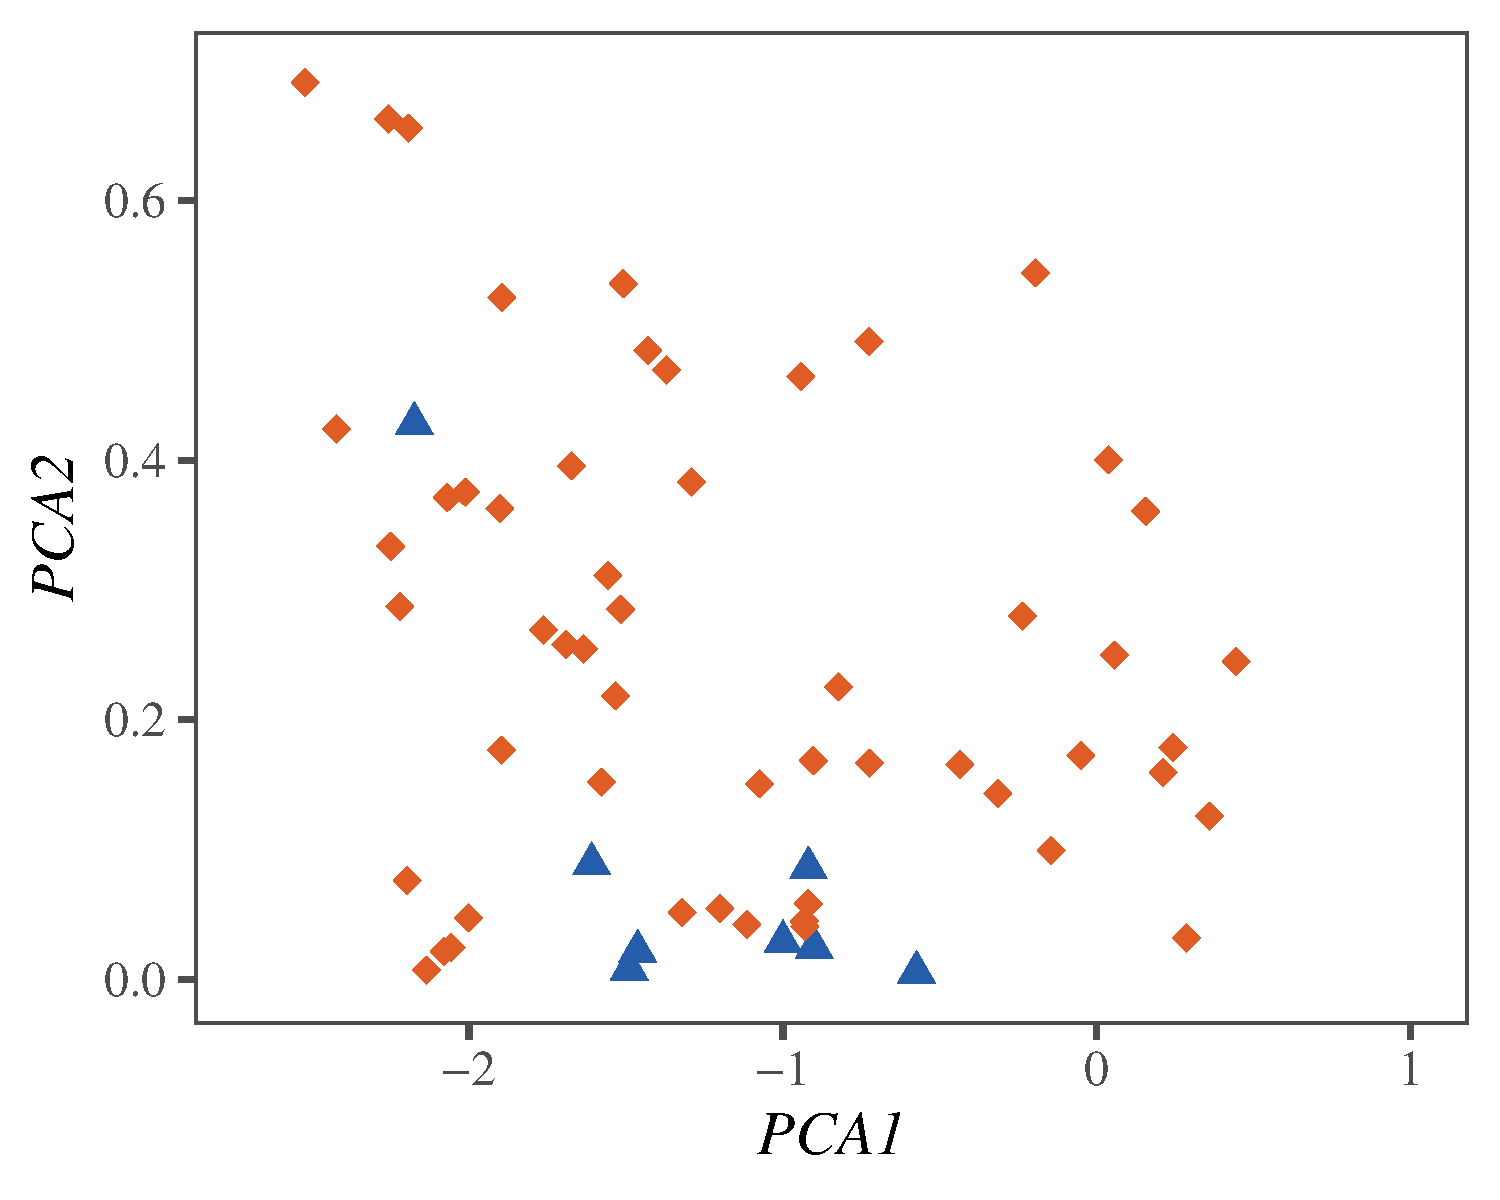
\includegraphics[width = .3\columnwidth]{Figures/GLCM.pdf}}
	\subfigure[SURF\label{Fig:surf}]{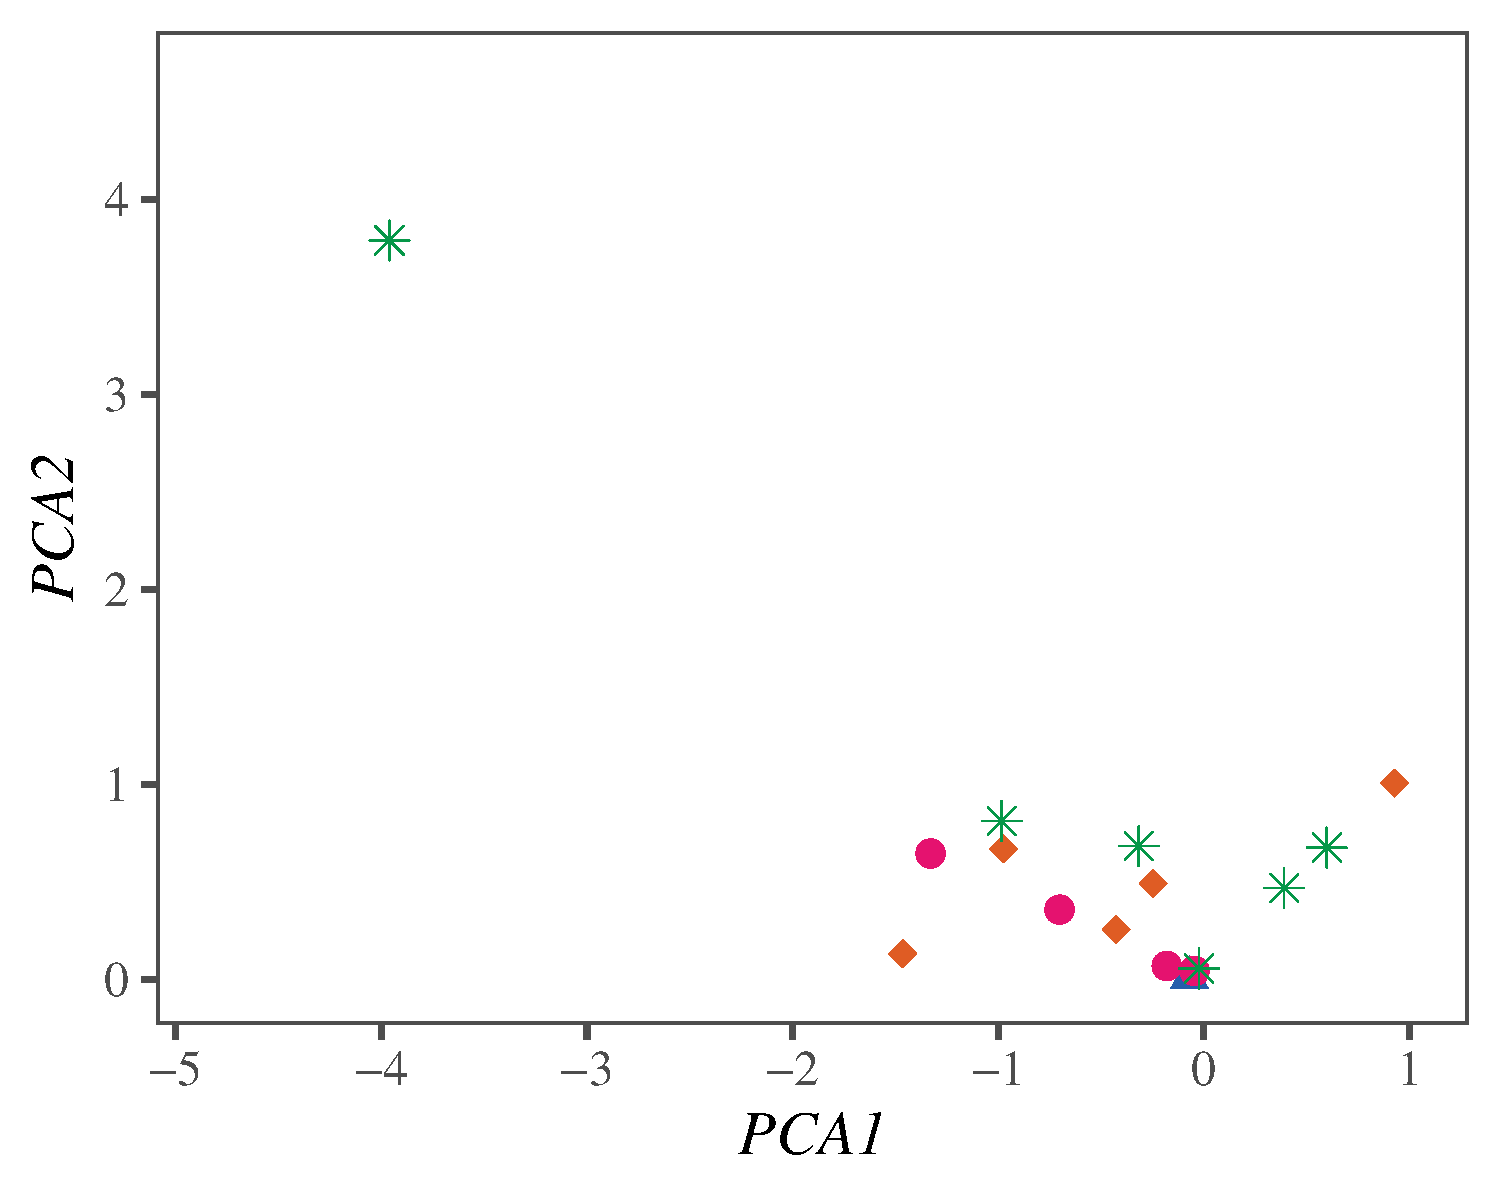
\includegraphics[width = .3\columnwidth]{Figures/Surf.pdf}}
	\subfigure[STFT + SURF\label{Fig:stft}]{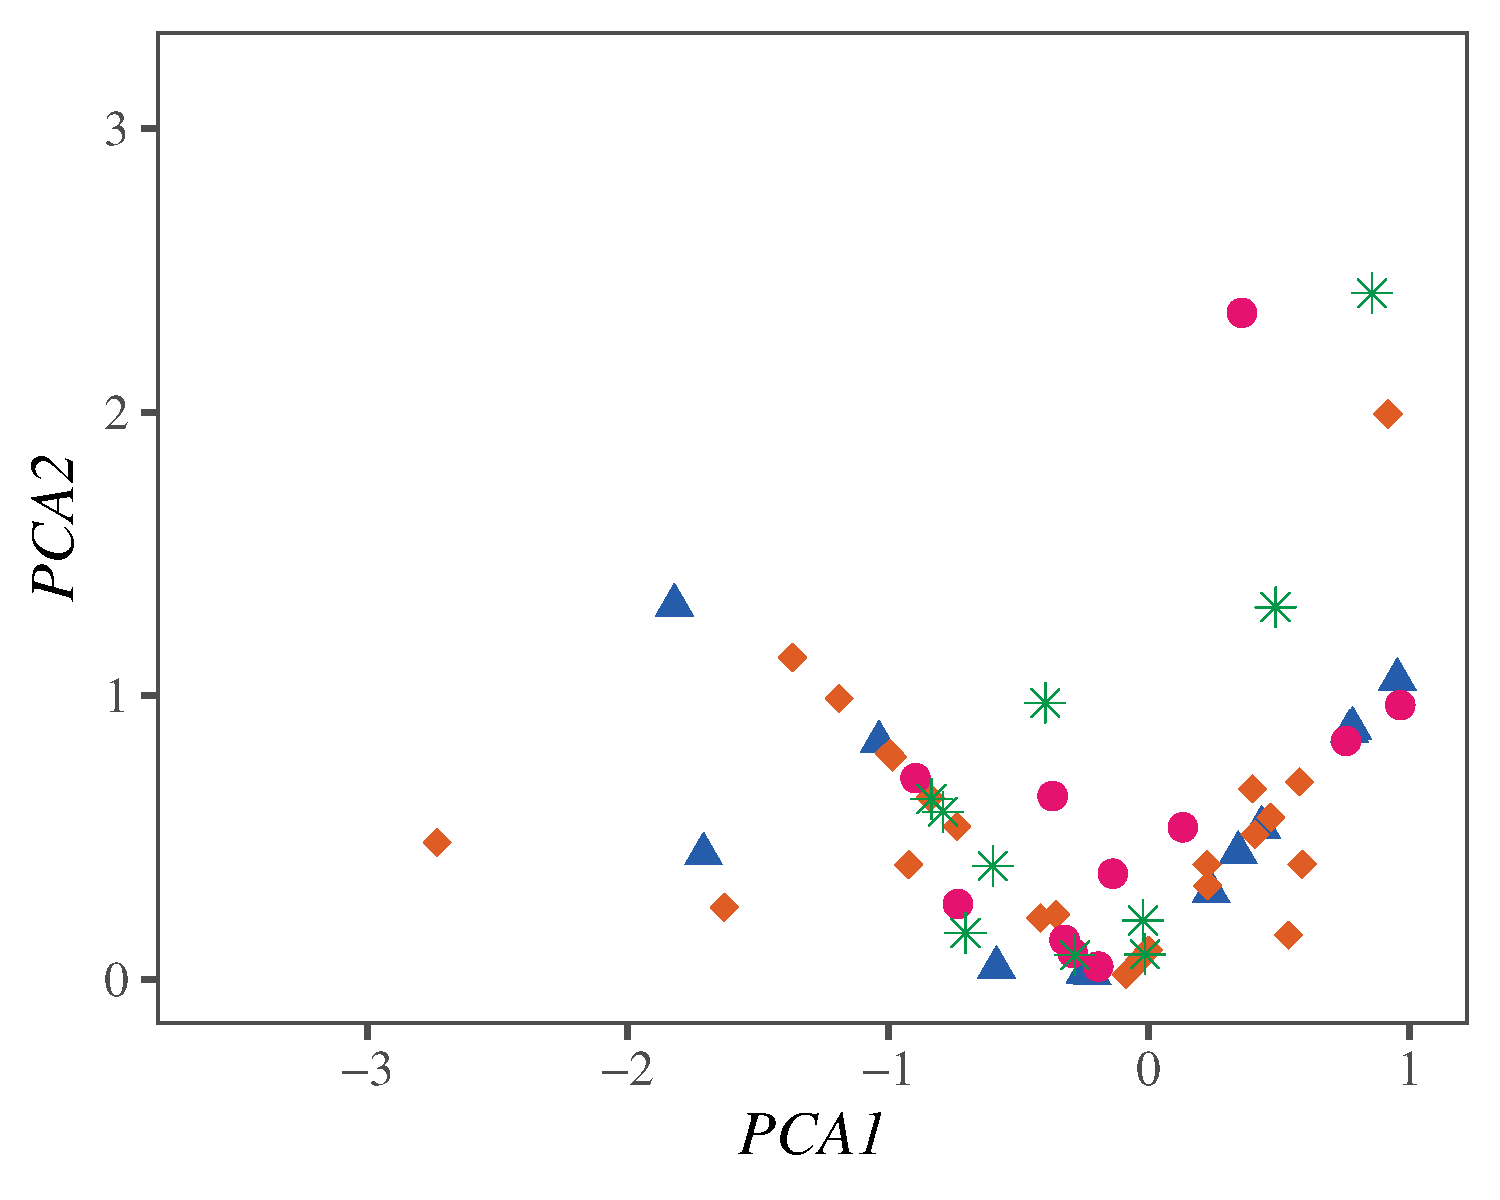
\includegraphics[width = .3\columnwidth]{Figures/StftSurf.pdf}}
	\subfigure[Bandt-Pompe\label{Fig:bp}]{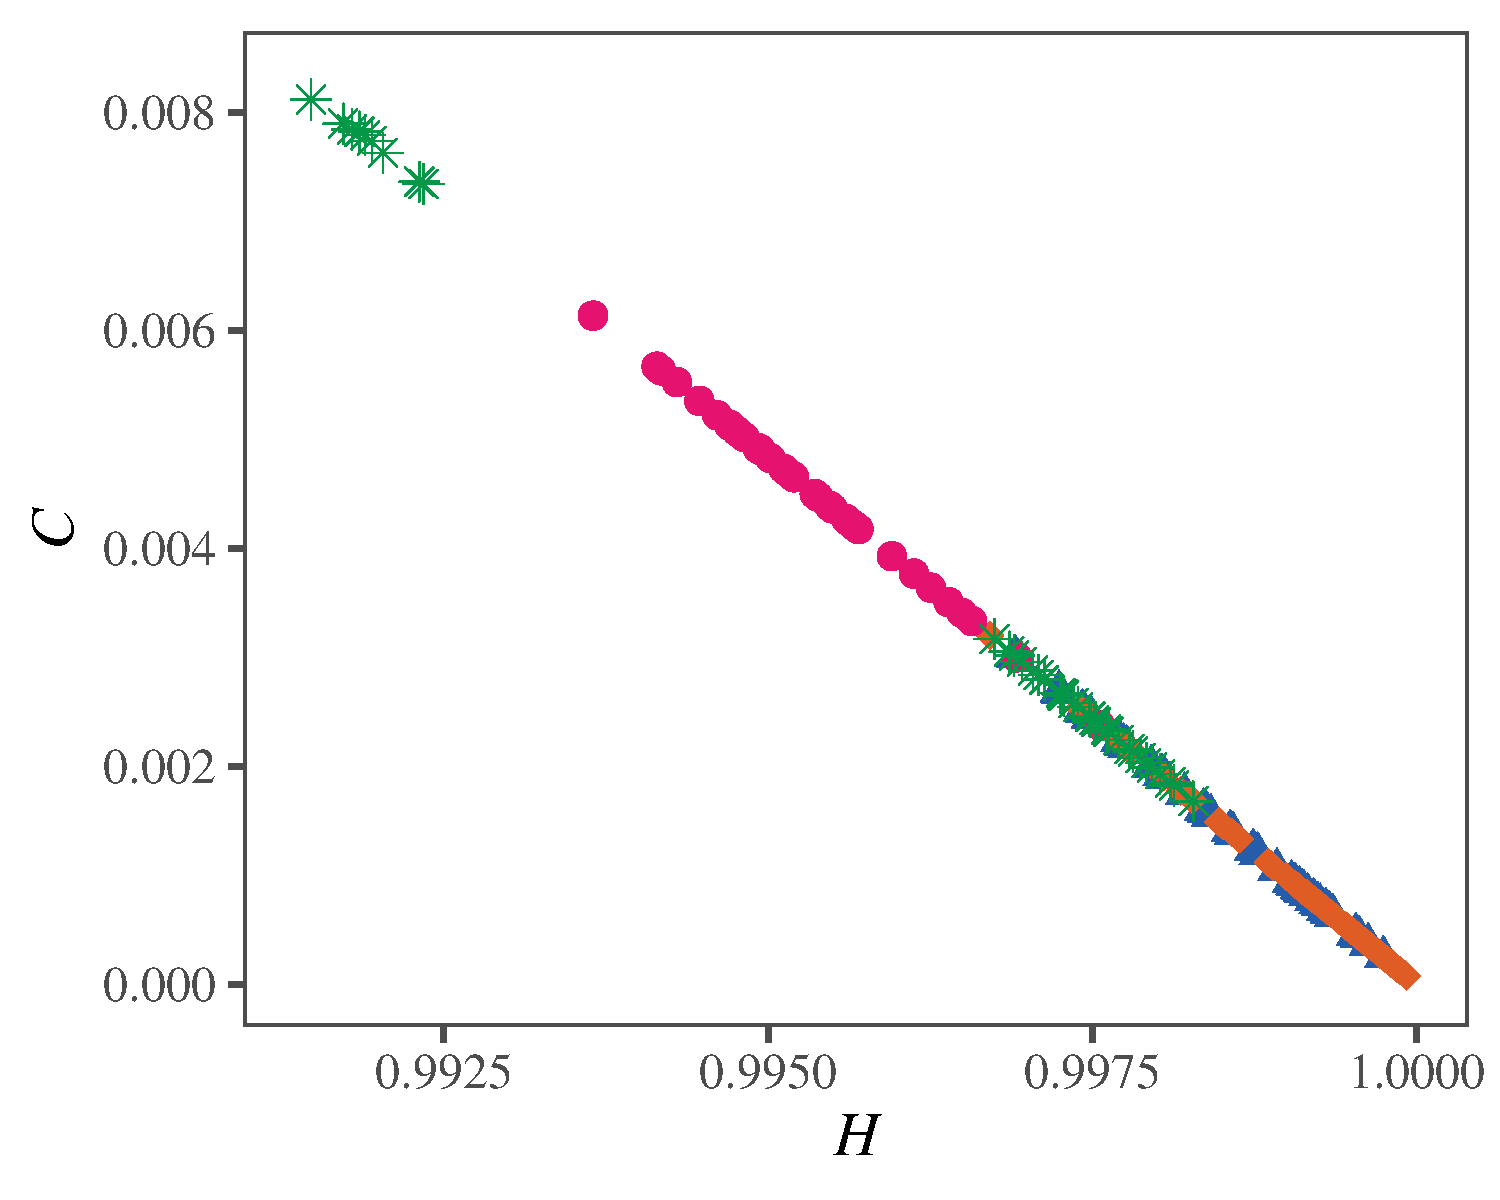
\includegraphics[width = .3\columnwidth]{Figures/BP.pdf}}
	\subfigure[Transition Graph\label{Fig:tg}]{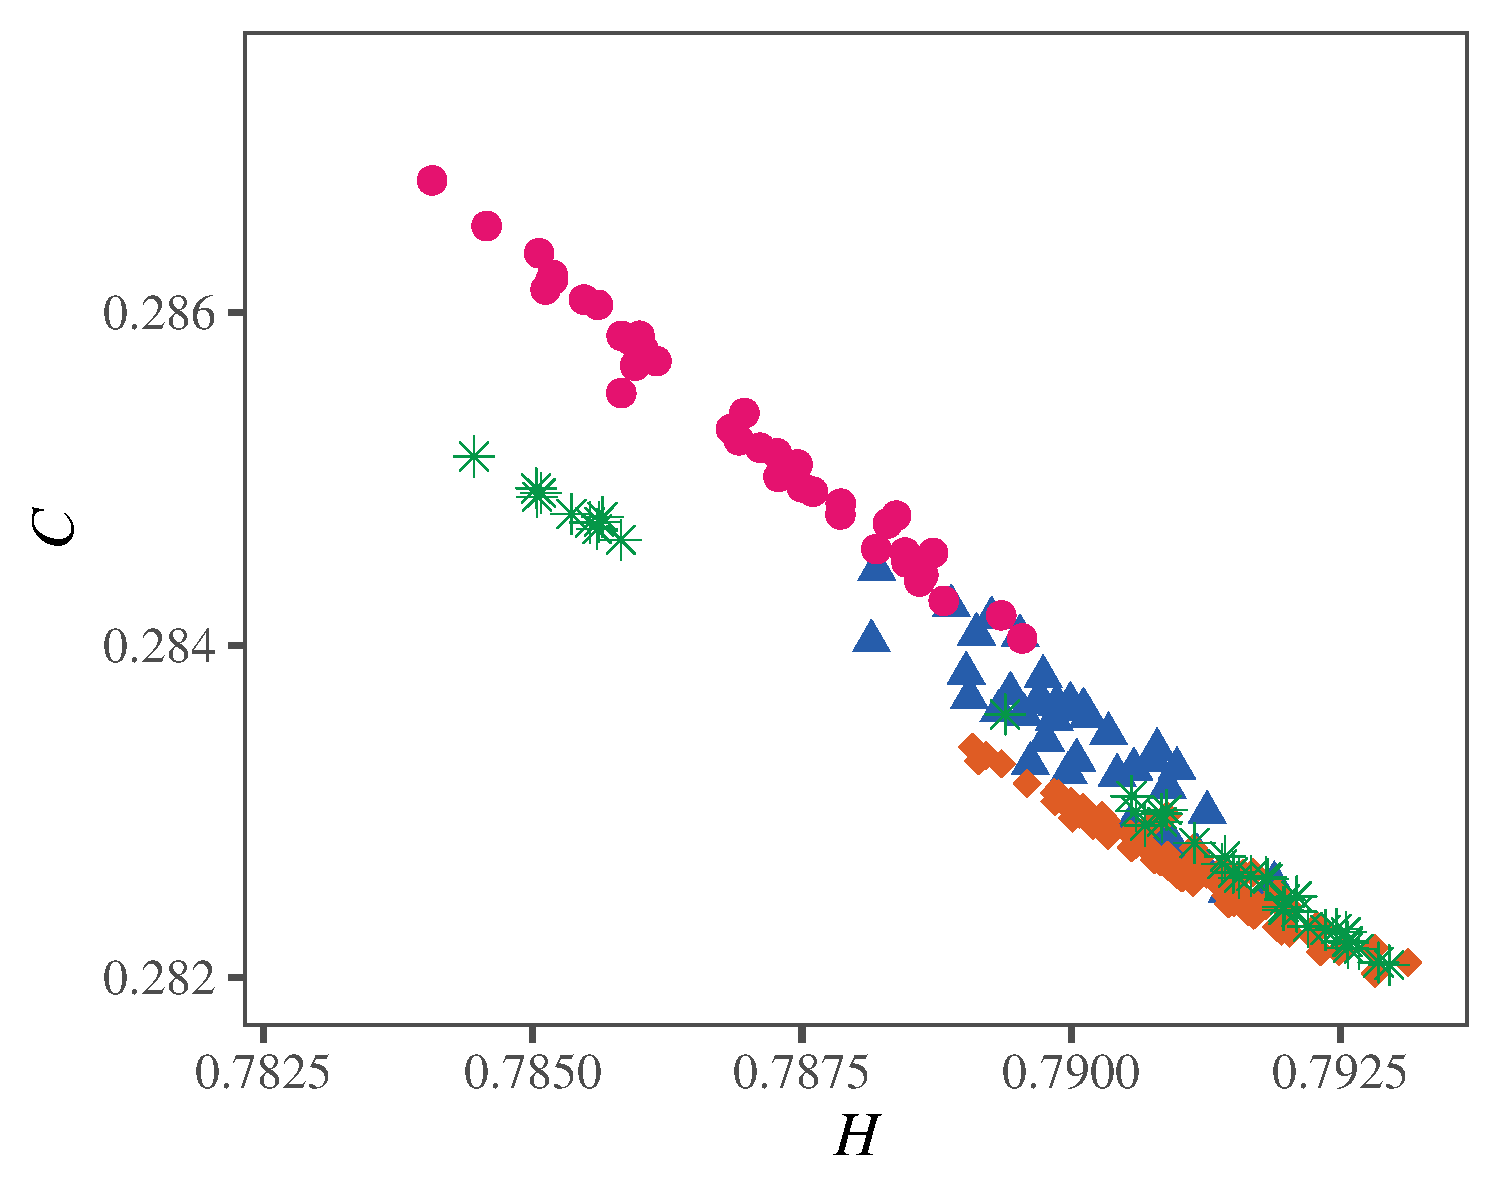
\includegraphics[width = .3\columnwidth]{Figures/TG.pdf}}
	\subfigure[WPE\label{Fig:wpe}]{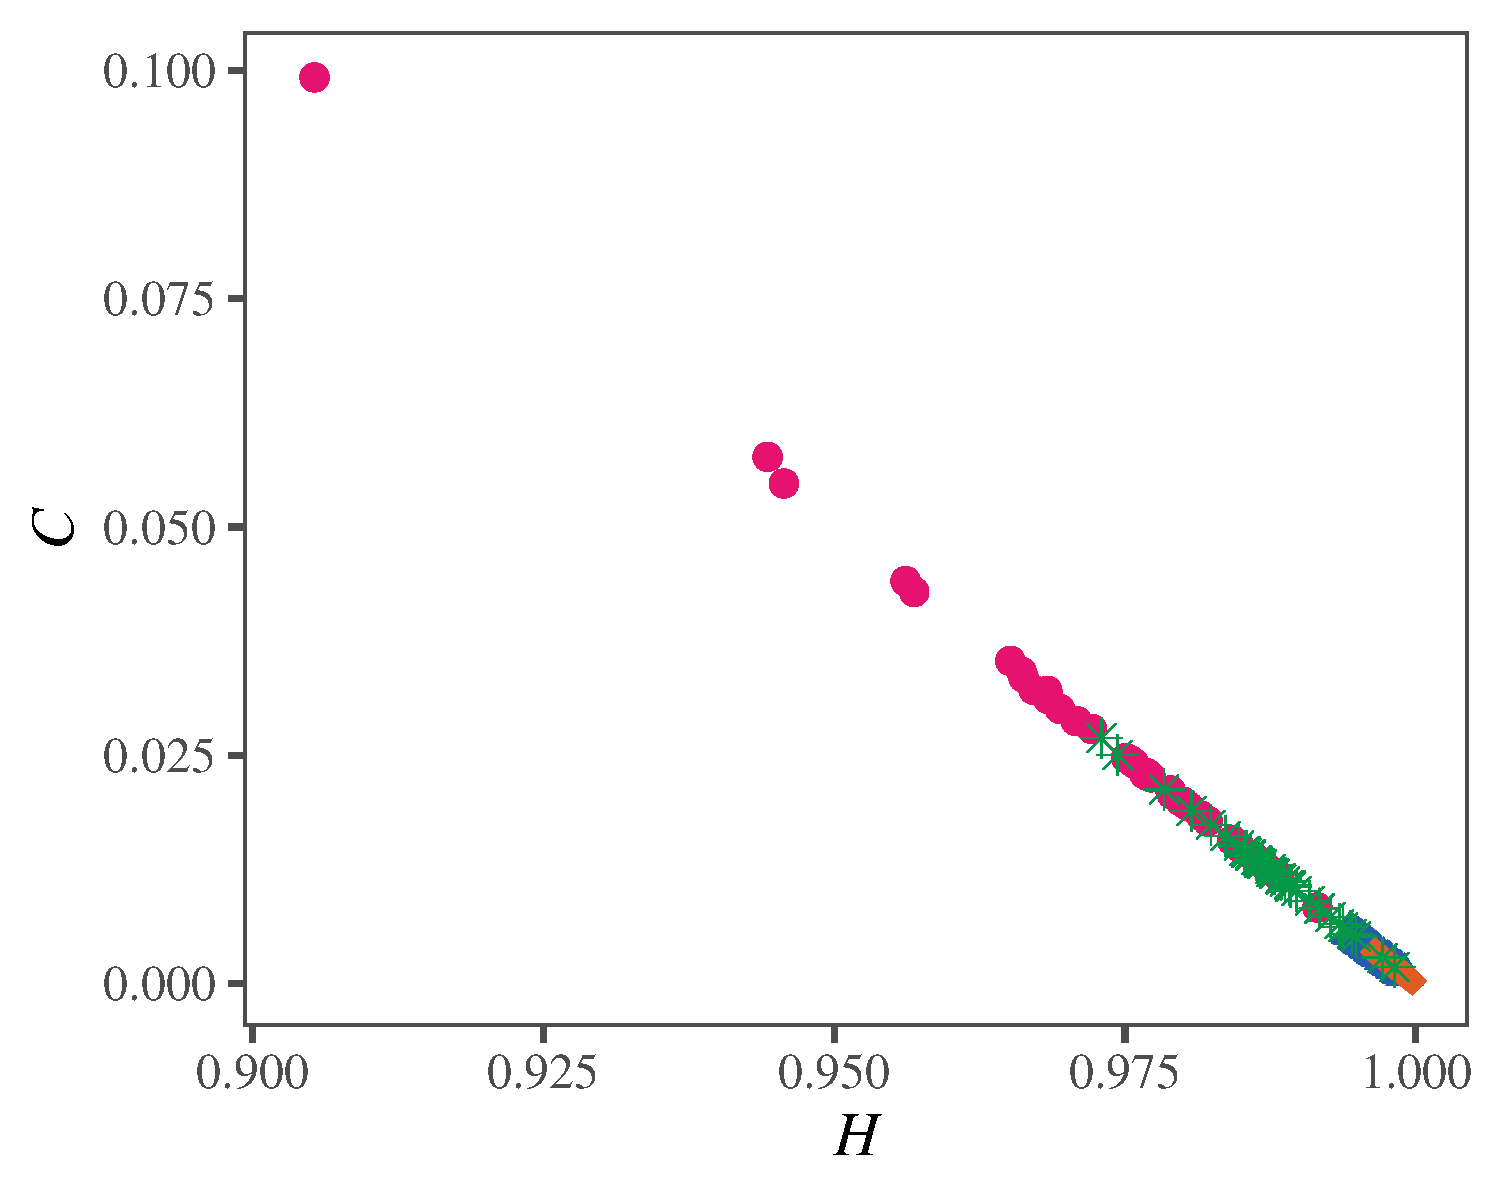
\includegraphics[width = .3\columnwidth]{Figures/WPE.pdf}}
	\subfigure[AAPE ($A = 0.5$)\label{Fig:aape}]{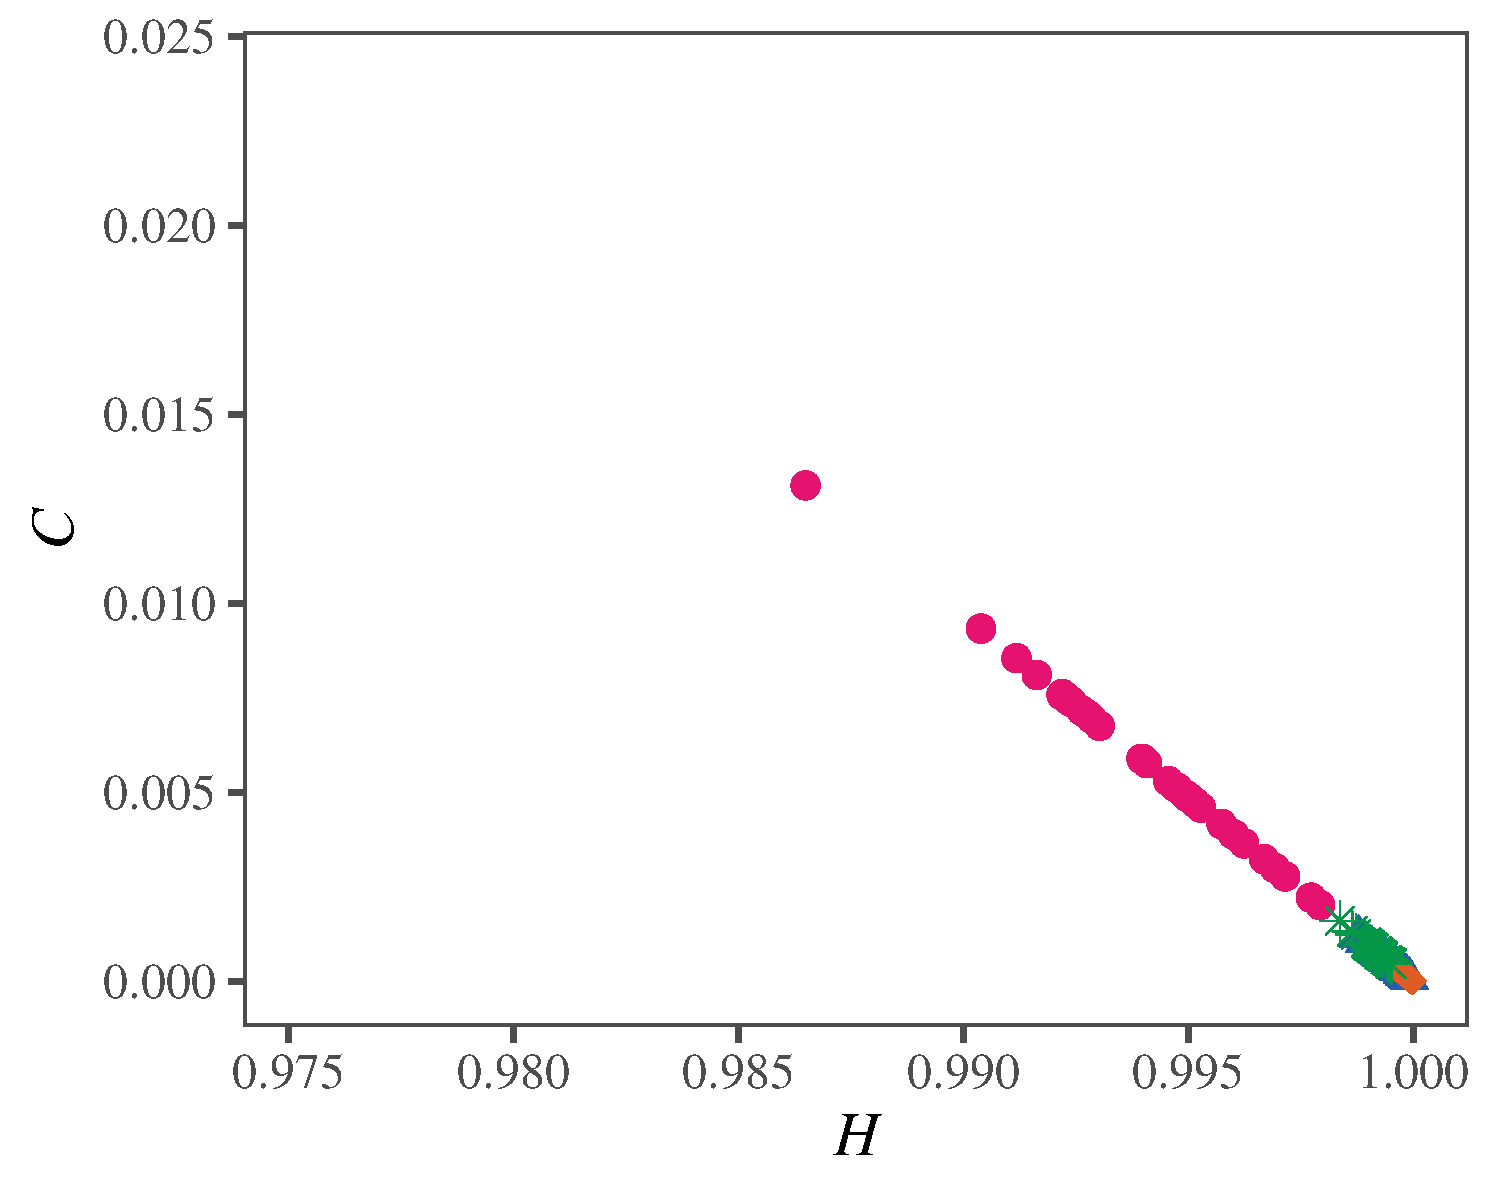
\includegraphics[width = .3\columnwidth]{Figures/AAPEA05.pdf}}
	\subfigure[FGPE ($\alpha = 0.5$)\label{Fig:fgpe}]{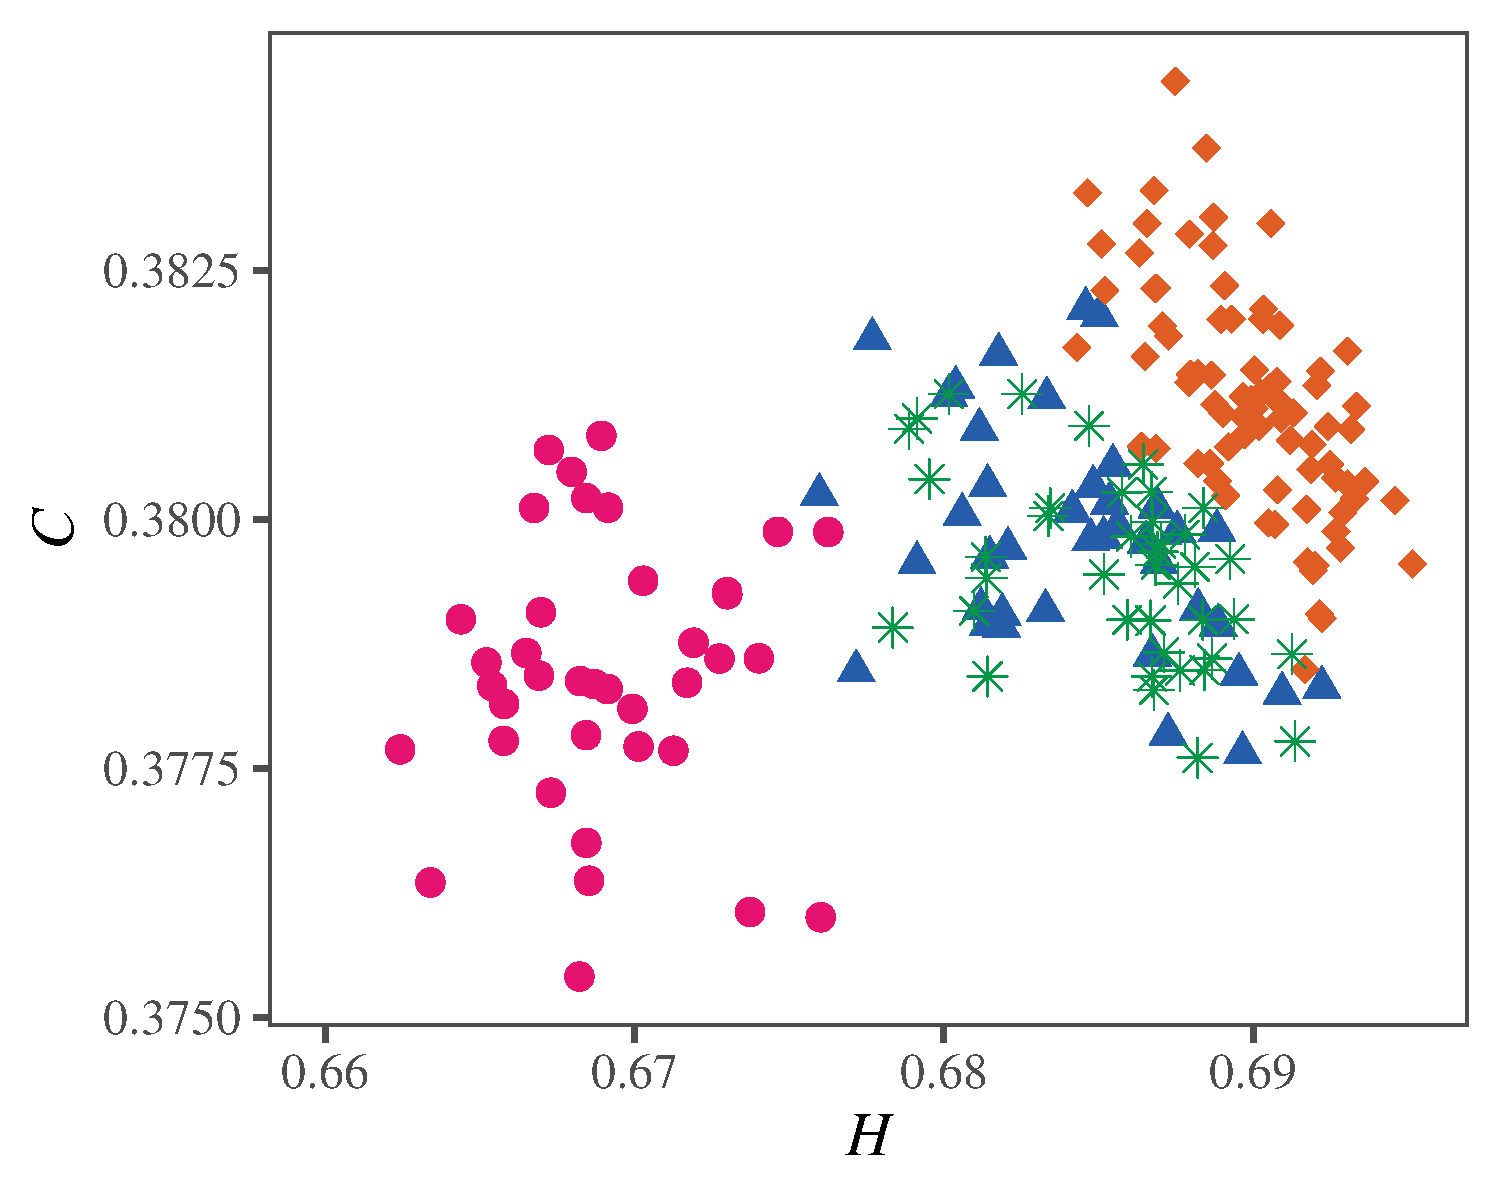
\includegraphics[width = .3\columnwidth]{Figures/FGPEA05.pdf}}
	\subfigure[WATG\label{Fig:watgD3T1}]{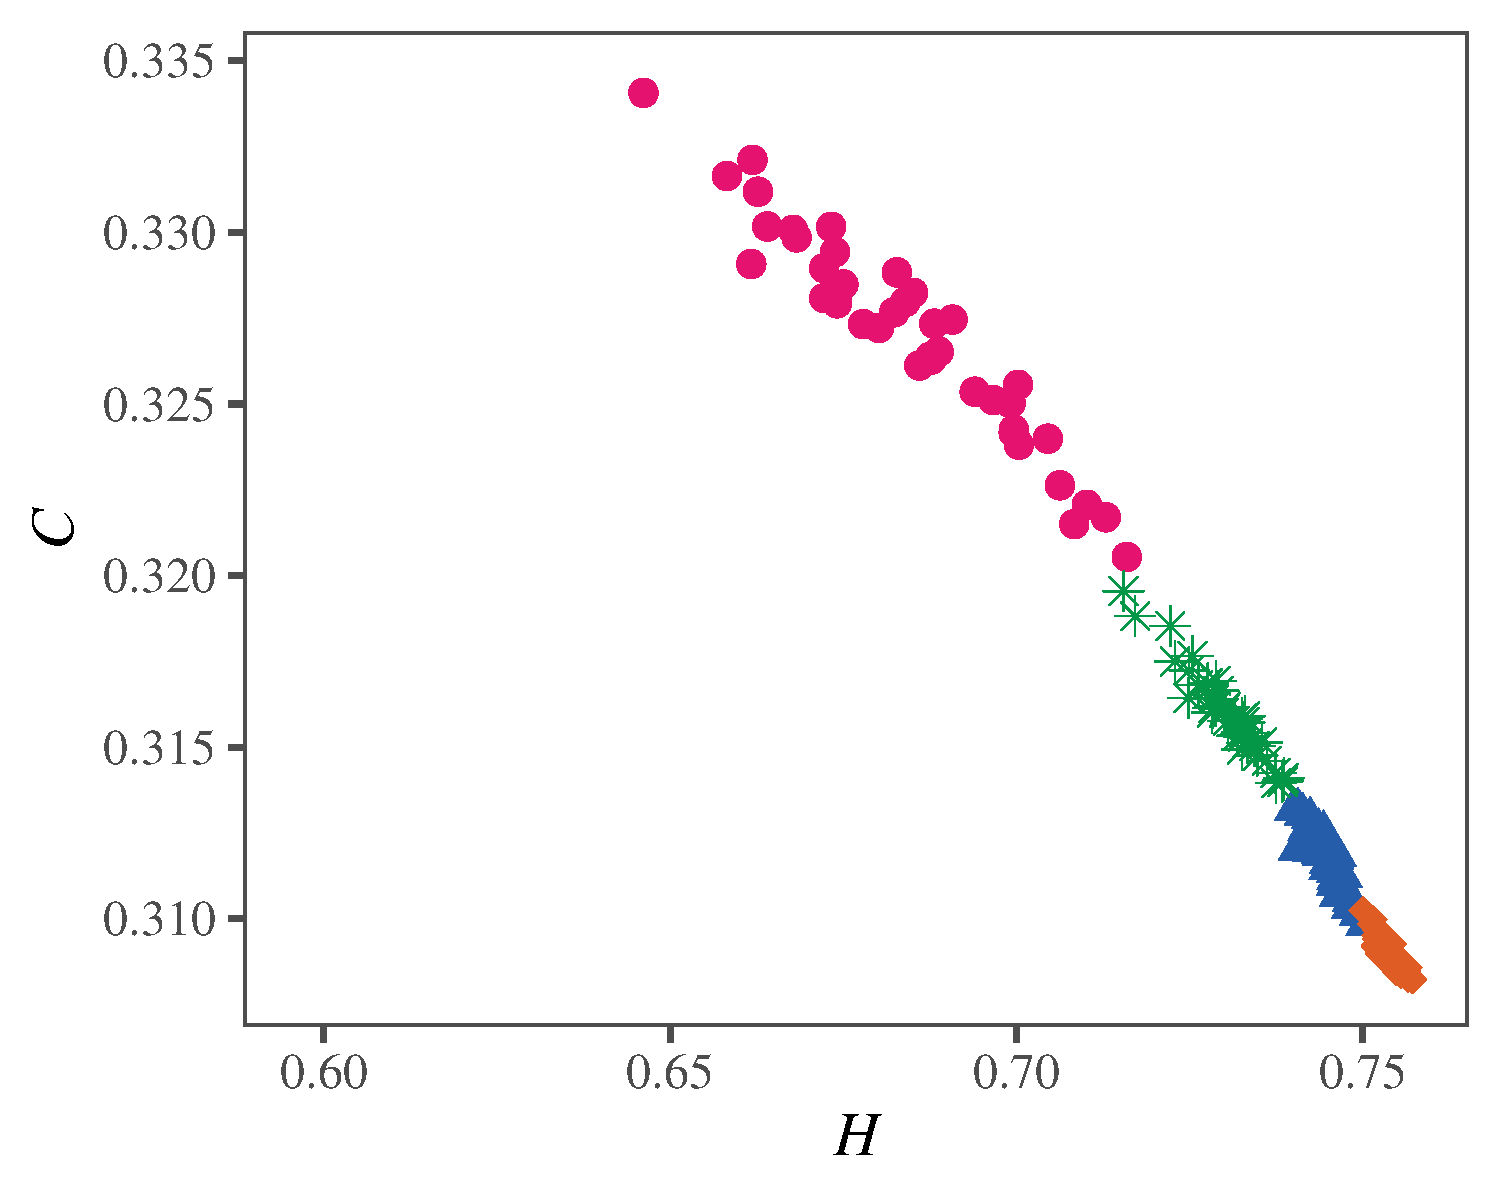
\includegraphics[width = .3\columnwidth]{Figures/WATG.pdf}}
	\caption{Bi-dimensional visualization of the descriptors obtained by our proposal and other methods of texture characterization and classification. 
	For those who provide more than two features, we apply the PCA algorithm to obtain such a visualization.}
	\label{fig:2DVisualization}
\end{figure*}

We classified the features using the $k$-nearest neighbor algorithm with Euclidean distance, selecting the value of $k$ with the automatic grid search method of the Caret R package~\cite{kuhn2008building}.
For validation, we used $10$-fold cross-validation.
More details about the classifier and the sampling can be seen in~\cite{mitchell1997machine}.

Table~\ref{tab:result1} presents the number of features each method produces, as well as its performance at classifying the $200$ samples.
We assessed the effectiveness of each approach using the following metrics. We used the first two metrics (Recall and Precision) to evaluate classifiers' per class performance and the last three metrics (Average Accuracy, Micro F1-score, and Macro F1-score) to evaluate the overall performance of the multi-class classifiers. We denote $\text{TP}_i$, $\text{TN}_i$, $\text{FP}_i$, and $\text{FN}_i$ as the true positives, true negatives, false positives, and false negatives counts of a given class $i$, among a set of $K$ classes, respectively.
\begin{itemize}
	\item Recall or True Positive Rate of the class $i$ (TPR$_i$): 
	\begin{equation*}
	\text{TPR$_i$} = \frac{\text{TP}_i}{\text{TP}_i + \text{FN}_i}.
	\end{equation*}
	%
	\item Precision or Positive Predictive Value of the class $i$ (PPV$_i$): \begin{equation*}
	\text{PPV$_i$} = \frac{\text{TP}_i}{\text{TP}_i + \text{FP}_i}.
	\end{equation*}
	%
	\item Average Accuracy (AA):
	\begin{equation*}
	\text{AA} = \sum^{\text{K}}_{i = 1}\left\{\frac{\text{TP}_i + \text{TN}_i}{\text{TP}_i + \text{TN}_i + \text{FP}_i + \text{FN}_i}\right\} 
	\end{equation*}
	%
	\item Micro F1-score: 
	\begin{equation*}
    	\text{PPV}_\mu = \frac{\sum^{\text{K}}_{i = 1}\text{TP}_i}{\sum^{\text{K}}_{i = 1}\text{TP}_i + \sum^{\text{K}}_{i = 1}\text{FP}_i}
	\end{equation*}
	\begin{equation*}
	    \text{TPR}_\mu =  \frac{\sum^{\text{K}}_{i = 1}\text{TP}_i}{\sum^{\text{K}}_{i = 1}\text{TP}_i + \sum^{\text{K}}_{i = 1}\text{FN}_i}
	\end{equation*}
	\begin{equation*}
	    \text{F1-score}_\mu = 2 \, \frac{\text{PPV}_\mu \times \text{TPR}_\mu}{\text{PPV}_\mu + \text{TPR}_\mu}.
	\end{equation*}
	%
	\item Macro F1-score: 
	\begin{equation*}
	\text{PPV}_M = \frac{1}{K} \sum^{\text{K}}_{i = 1}\frac{\text{TP}_i}{\text{TP}_i + \text{FP}_i}
	\end{equation*}
	\begin{equation*}
	\text{TPR}_M =  \frac{1}{K} \sum^{\text{K}}_{i = 1}\frac{\text{TP}_i}{\text{TP}_i + \text{FN}_i}
	\end{equation*}
	\begin{equation*}
	\text{F1-score}_M = 2 \, \frac{\text{PPV}_M \times \text{TPR}_M}{\text{PPV}_M + \text{TPR}_M}.
	\end{equation*}
\end{itemize}

\begin{table}
	\centering
	\caption{Experimental results using $k$-NN}
	\label{tab:result1}
    \scalebox{0.65}{
	\begin{tabular}{lrrrr*9{r}}
		\toprule
		\multirow{2}{*}{Method} & \multirow{2}{*}{\# features} & & TPR & & & & PPV & & & \multirow{2}{*}{AA} & \multirow{2}{*}{$\text{F1-Score}_{\mu}$} & \multirow{2}{*}{$\text{F1-Score}_M$} \\ 
		\cmidrule(lr){3-6} 
		\cmidrule(lr){7-10}
		&   & Forest & Pasture & Ocean & Urban & Forest & Pasture & Ocean & Urban & &  \\ 
		\cmidrule(lr){1-1}
		\cmidrule(lr){2-2}
		\cmidrule(lr){3-6}
		\cmidrule(lr){7-10}
		\cmidrule(lr){11-11}
		\cmidrule(lr){12-12}
		\cmidrule(lr){13-13}
		Gabor & 80 & 
		1.000 & 1.000 & 1.000 & 1.000 & 
		1.000 & 1.000 & 1.000 & 1.000 & 
		1.000 & 1.000 & 1.000\\
		HOG & 54 & 
		1.000 & 1.000 & 1.000 & 1.000 & 
		1.000 & 1.000 & 1.000 & 1.000 & 
		1.000 & 1.000 & 1.000\\
		GLCM & 32 & 
		0.833 & 1.000 & 1.000 & 0.833 &
		1.000 & 0.857 & 0.923 & 1.000 &
		0.967 & 0.980 & 0.970\\
		SURF & 1856 & 
		0.500 & 0.000 & 1.000 & 0.000 & 
		1.000 & 0.000 & 0.444 & 0.000 &
		0.467 & 0.666 & 0.572\\
		STFT + SURF  & 1856 & 
		0.166 & 0.000 & 0.833 & 0.166 & 
		0.250 & 0.000 & 0.416 & 0.500 &
		0.300 & 0.462 & 0.292\\
		\cmidrule(lr){1-1}
		\cmidrule(lr){2-2}
		\cmidrule(lr){3-6}
		\cmidrule(lr){7-10}
		\cmidrule(lr){11-11}
		\cmidrule(lr){12-12}
		\cmidrule(lr){13-13}
		Bandt-Pompe & 2 & 
		0.333 & 1.000 & 0.750 & 1.000 &
		0.500 & 0.857 & 0.750 & 0.857 &
		0.600 & 0.776 & 0.633\\ 
		Transition Graph & 2 & 
		0.833 & 0.666 & 0.833 & 1.000 &
		0.833 & 0.800 & 0.769 & 1.000 &
		0.767 & 0.929 & 0.875\\
		\cmidrule(lr){1-1}
		\cmidrule(lr){2-2}
		\cmidrule(lr){3-6}
		\cmidrule(lr){7-10}
		\cmidrule(lr){11-11}
		\cmidrule(lr){12-12}
		\cmidrule(lr){13-13}
		WPE & 2 & 
		1.000 & 0.833 & 1.000 & 0.833 &
		0.857 & 0.833 & 1.000 & 1.000 &
		0.933 & 0.868 & 0.779\\ 
		AAPE & 2 & 
		0.666 & 1.000 & 1.000 & 1.000 &
		1.000 & 0.857 & 0.923 & 1.000 &
		0.833 & 0.947 & 0.896\\ 
		FGPE & 2 & 
		0.666 & 0.666 & 1.000 & 1.000 &
		0.800 & 0.666 & 0.923 & 1.000 &
		0.767 & 0.868 & 0.711\\ 
		\cmidrule(lr){1-1}
		\cmidrule(lr){2-2}
		\cmidrule(lr){3-6}
		\cmidrule(lr){7-10}
		\cmidrule(lr){11-11}
		\cmidrule(lr){12-12}
		\cmidrule(lr){13-13}
		WATG & 2 & 
		1.000 & 1.000 & 1.000 & 1.000 &
		1.000 & 1.000 & 1.000 & 1.000 &
		1.000 & 1.000 & 1.000\\
		\bottomrule
	\end{tabular}}
\end{table}

Table~\ref{tab:result1} shows that, among the methods of weighting ordinal patterns, FGPE produced the worst results: $\text{AA} = \SI{76.7}{\percent}$, $\text{F1-score}_\mu = \SI{86.8}{\percent}$, and $\text{F1-score}_M = \SI{71.1}{\percent}$.
%
WPE also produced a low F1-score, but it produced consistently better results in the other metrics, presenting $\text{AA} = \SI{93.3}{\percent}$.
%
AAPE achieved one of the best F1-score results: $\text{AA} = \SI{83.3}{\percent}$, $\text{F1-score}_\mu = \SI{94.7}{\percent}$, and $\text{F1-score}_M = \SI{89.6}{\percent}$.
%
WATG, considering the transition graph of ordinal patterns, can better describe the textures presented, as it achieves the best performance achievable in all metrics: \SI{100}{\percent}.

\mbox{STFT + SURF} produced the worst results: $\text{AA} = \SI{30.0}{\percent}$, $\text{F1-score}_\mu = \SI{46.2}{\percent}$, and $\text{F1-score}_M = \SI{29.2}{\percent}$.
%
SURF alone provided a better performance: $\text{AA} = \SI{46.7}{\percent}$,  $\text{F1-score}_\mu = \SI{66.6}{\percent}$, and $\text{F1-score}_M = \SI{57.2}{\percent}$.
%
HOG and Gabor filters achieved the highest success rates
among all the handcrafted methods here considered: $\text{AA} = \SI{100}{\percent}$, $\text{F1-score}_\mu = \SI{100}{\percent}$, and $\text{F1-score}_M = \SI{100}{\percent}$.
However, WATG achieves that same performance using only $2$ features.
This reduction implies less computational power requirement and avoids the curse of dimensionality~\cite{TheCursesofDimensionality2018}.
Moreover, the features it is based upon are fully interpretable.

\section{Conclusions}\label{Conclusion}

We presented and assessed a new method of analysis and classification of SAR image textures.
This method consists of three steps: 
(1)~linearization, 
(2)~computing the Weighted Ordinal Pattern Transition Graph, and 
(3)~obtaining Information Theory descriptors.
A simple $k$-NN algorithm applied to the pairs Entropy-Statistical~Complexity classifies the data with \SI{100}{\percent} performance.
In addition to such perfect separation among urban, pasture, ocean, and forest areas, the proposed descriptors are interpretable in terms of the degree and structure of the spatial dependence among observations.

Experiments using patches from UAVSAR images showed that the proposal performs better than GLCM, Bandt-Pompe, Transition Graphs, SURF, \mbox{STFT + SURF}, and other techniques which also employ amplitude information in the analysis of ordinal patterns. 
Our approach provides the same quality of results obtained with Gabor filters and HOG.
However, while Gabor filters employ $80$ features and HOG uses $54$ features, our proposal requires only two.
This such reduced dimensionality consists of a huge advantage over the other techniques, with added values:
Firstly, by reducing the dimension of the features to \mbox{2-D}, we can visualize the differences between the classes of regions analyzed.
Secondly, for machine learning algorithms, the smaller the number of dimensions, the faster the training process is, and the less storage space is required.
Thirdly, we managed to avoid overfitting, a recurring problem in data with high dimensionality.

We also observed that only one feature ($H$ or $C$) is enough to discriminate the classes with the same reported performance. We opted to preserve both features because we consider that this study shed light on a novel way of SAR image analysis. Thus, we preferred to stick to the most common ordinal pattern analysis using the $H \times C $ plane. 
As future work, we consider investigating the discriminative power of these features in more complex situations.

Our approach is robust to rotations and the presence of speckle noise. The behavior showed in Figure~\ref{Fig:TestSpeckleHC} shows that our approach can capture the speckle contamination adequately.

Since the application of this work is limited to texture patches from homogeneous regions, we aim to study the possible impacts of heterogeneous areas, such as mixed culture and urban regions.
	
\section{Reproducibility and Replicability} 

Following the guidelines presented in Ref.~\cite{ABadgingSystemforReproducibilityandReplicabilityinRemoteSensingResearch}, the text, source code, and data used in this study are available at the \textit{SAR-WATG} repository \url{https://github.com/EduardaChagas/SAR-WATG}.
The information includes a link to download the $200$ labeled samples we employed in the analysis.